\chapter{Results}
\label{Results}

This chapter works through the method described in section \ref{Method}, commenting on the results and providing a brief discussion of their immediate interpretation. The chapter begins with the creation of the correlation matrices, and works through to the results of the model implementation. There are 8 clusters including the catch all Soup Node, the clusters are defined by by the peak hour which is the only point the mean load profile of each cluster is significantly different from 0kWh.  The results show that the approach developed for predicting day ahead load profile using clustered smart meters, is an effective method of prediction, with a MAPE of 3.9\%, outperforming the linear predictor and having a similar MAPE score to the models used in the literature.

The classification model that predicts the cluster of each individual node produced a model whose interpretation was more mixed, it accurately predicts the correct cluster 25\% and with a low kappa score indicates that the model is not predictive. The two XGboost models the simple model with the same information and the expanded model with the previous weeks clusters performed similarly, the expanded had slightly better metric with an accuracy of  0.3689 and $\kappa$ of 0.178, which is still not very strong. Part of the reason for this poor classification performance is, that predicting in a similar time period results in a miss-classification even though the real difference is small. The low levels of consistent behaviour shown in \ref{fig:MeanAbsCorr} would suggest that predicting day ahead behaviour at node level would be challenging.  The socio-demographic detection model showed random behaviour and no predictive power this may be because it suffers from inaccuracies inherent to the MOSAIC method which is specific to an area but not a household, or simply because there is no link between socio-demographic class and electricity consumption.


\section{Creating correlation matrices} \label{sec:CormatEdge}
As there are 5260 nodes in the dataset the resulting matrix contained 2.7 million elements, of varying degree's of correlation, this structure can then be represented in a graph, the ordered correlation matrix is shown in figure \ref{fig:day100corplot}. By creating the correlation matrices for all days, it reduces the computational load for making changes later on in the processing pipeline, such as changing the minimum correlation requirements for link and rebuilding the graphs. Each correlation matrix was over 200mb matrix, together the total size of all the correlation matrices was over 40Gb.

\begin{figure}
    \centering
    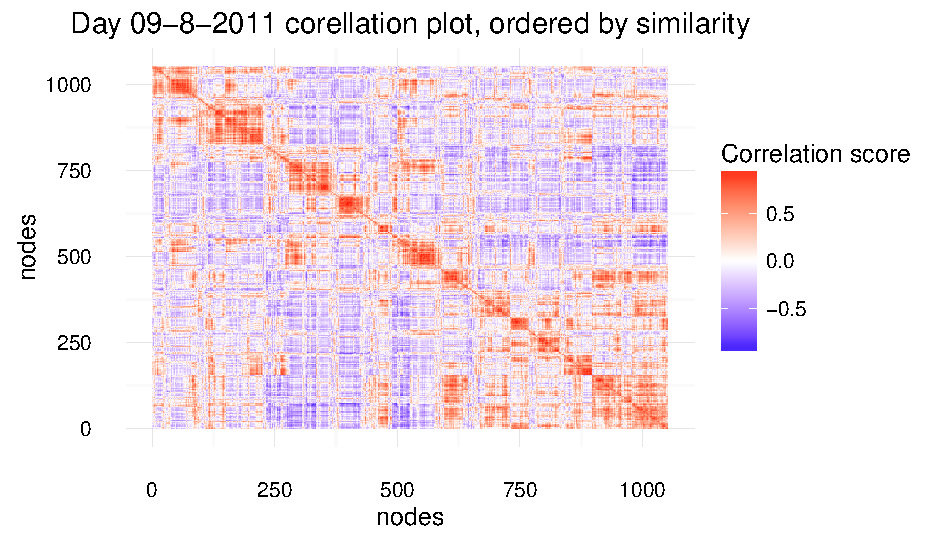
\includegraphics[width=\textwidth]{Figures/Results/day100Corplot}
    \caption[Example corellation matrix]{The correlation matrix of 09-08-2011 with the nodes organised by hierarchical similarity.}
    \label{fig:day100corplot}
\end{figure}

\section{Finding an appropriate  edge correlation cut off point}
The results of edge analysis are shown in figure \ref{fig:EdgeNodeAnalysis}. They reveal that that the number of edges and non-isolated nodes are relatively consistent across the graphs. Subfigure \ref{fig:Meanedges} shows that the number of edges decreases approximately quadratically with increasing minimum correlation. It can be seen that there is a small right skew in the data as there is a visible difference between the mean and the median, the standard deviation of the edge number is approximately 10\% of the mean. 

Sub figure \ref{fig:Meannodes} shows the mean number of nodes for each cut off point. Node number analysis showed very little variation with a negligible standard deviation and a median that is the same as the mean. It is clear that the total number of non-isolated nodes stays almost constant up to quite high levels of correlation before dropping off steeply to zero. Comparing the percentage of non-isolated nodes against the percentage of total edges as in \ref{fig:Edgenodeperc} shows that the percentage difference between the two grows quite large, figure \ref{fig:EdgeNodeDiff} shows the difference is maximised at a cut off of 0.8. 

The results of this analysis suggests that using 0.8 as a cut off will provide the highest number of non-isolated nodes for the lowest number of edges. However it should be noted that although the number of non-isolated nodes is low, experimenting with various graphs reveals that there are many nodes in small unconnected sub graphs of two or three, therefore the cut off point will be set at a more conservative 0.7. This makes a much more highly connected graph but is still tractable. 

With the cut off point chosen at 0.7 all graphs can be generated and community detection performed.

\begin{figure*}[ht]
\centering
\textbf{Number of edges analysis}\par\medskip
\subfloat[]{
  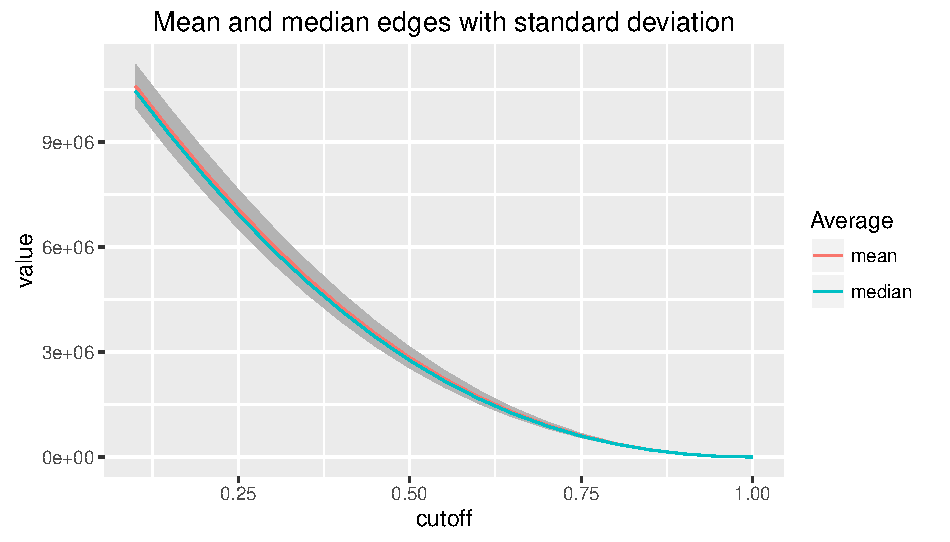
\includegraphics[width=0.49\textwidth]{Figures/Results/Meanedges}\label{fig:Meanedges}
}
\subfloat[]{
  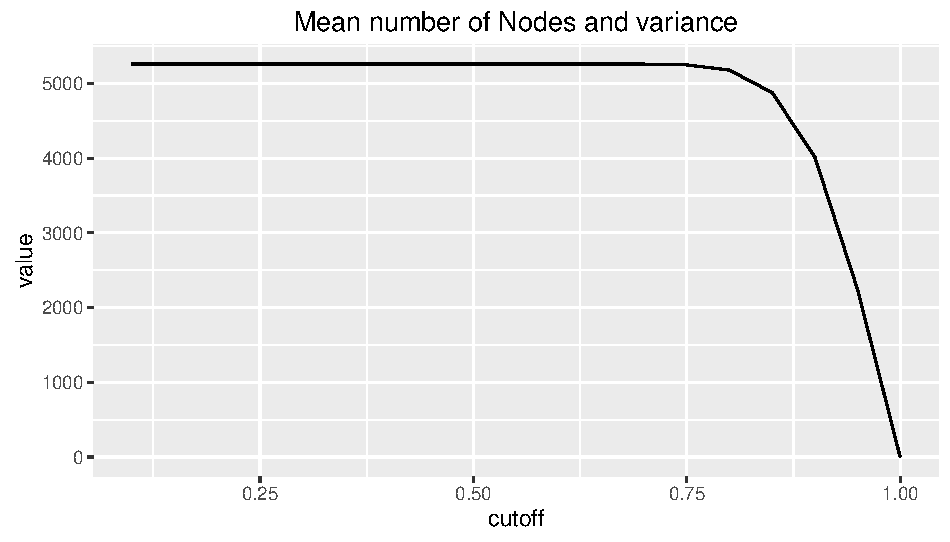
\includegraphics[width=0.49\textwidth]{Figures/Results/Meannodes}\label{fig:Meannodes}
}

\subfloat[]{
  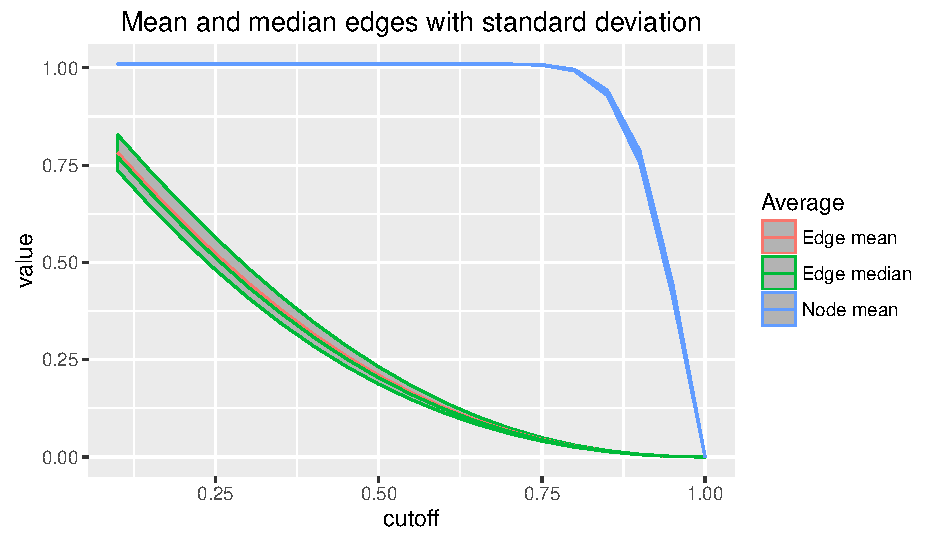
\includegraphics[width=0.49\textwidth]{Figures/Results/Edgenodeperc}\label{fig:Edgenodeperc}
}
\subfloat[]{
  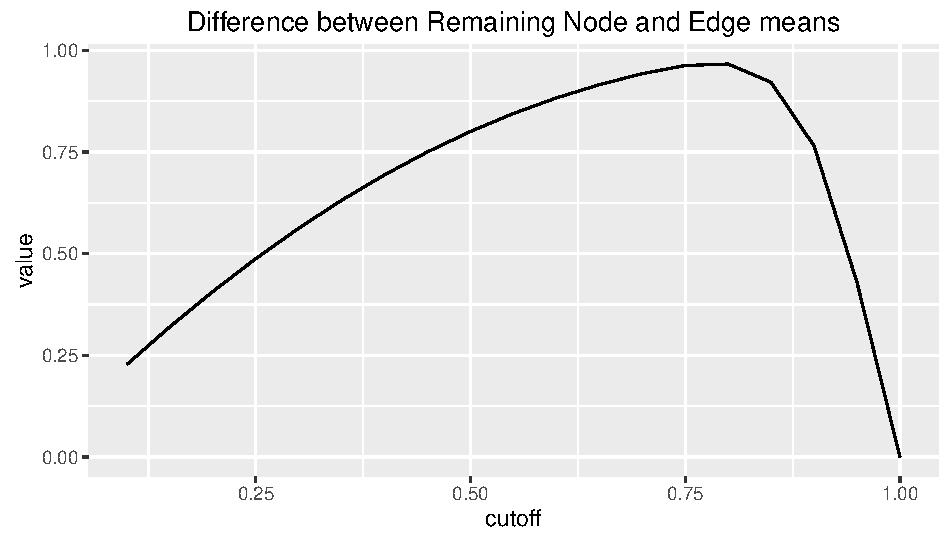
\includegraphics[width=0.49\textwidth]{Figures/Results/EdgeNodeDiff}\label{fig:EdgeNodeDiff}
}
\caption[Number of edges analysis]{Analysis of the number of edges and nodes for given correlation cut offs, across all 233 days, shows a relatively low standard deviation and slight skew with the number of edges. The number of nodes has an extremely low standard deviation, comparing the difference between the percentage remaining nodes and edges sees that the value is maximised at a correlation cut off of about 0.8. }
\label{fig:EdgeNodeAnalysis}
\end{figure*}


\subsection{Comparison with an Erdos-Renyi graph}

It is interesting to see if the the graph has a significantly different number of non-isolated nodes than an ER (Erdos-Renyi) graph for the same number of edges. This test was done by generating 20 different ER graphs with the same number of edges as the mean number of edges for each cut off point for the smart meter data. The mean number of non-isolated nodes were then compared with the mean number from the smart meter data, a plot comparing the results can be seen in \ref{fig:DataVsER}. A paired T-test was performed on the ER and smart meter non-isolated nodes. It rejected the NULL hypothesis that the mean difference between the graph types is zero with a p-value of 0.13, well above the 5\% confidence limit, there was an average difference of approximately 270 nodes. The ER graph had 0 variance for missing nodes for almost the entire test, dropping to zero on the last cut off point, this is shown in figure \ref{fig:DataVsER}. 

\begin{figure}[ht]
    \centering
    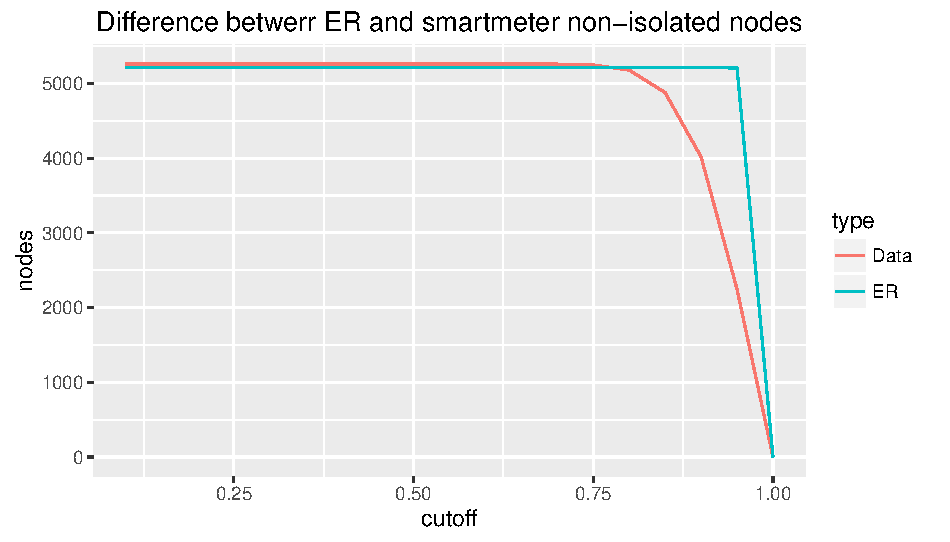
\includegraphics{Figures/Results/DataVsER}
    \caption[ER \& Data edge comparison]{There is a clear difference between the mean number of non-isolated nodes in an ER graph and the dataset. The drop-off point for the ER graph comes at some point after the 0.95 cut off.}
    \label{fig:DataVsER}
\end{figure}

\section{Creating the graphs}
Once the correlation matrices were constructed the graphs could be created, each graph was about 50Mb meaning all graphs totalled approximately 10Gb of storage space. As was seen from \ref{sec:CormatEdge} the number of edges and connected nodes drops off dramatically with a linear increase in minimum correlation requirement, this is confirmed by the graphs shown in figure \ref{fig:cutoff70vs90}, which compares a correlation requirement of 0.9 and 0.7. For ease of interpretation all unconnected nodes have been removed from the image. Figure \ref{fig:day100-90} has considerably fewer nodes than \ref{fig:day100-70} and is in comparison sparsely connected, the result is that the two images look entirely unrelated when they are in fact based on the same day with only a 0.2 change in correlation requirement. 

Another point of interest in the image is to see how communities are located within the graph as figure \ref{fig:day100-90} is much more sparse it is easier to see how the nodes are related to each other. It can be seen that clusters can form where nodes can be more related to a neighbouring cluster than to far away members of their own cluster. Ideally all cluster members are highly connected to the other members of their cluster and less to nodes outside the cluster, however as seen in the figure this may not always be the case. Cluster shape and spread is linked to modularity as described in \ref{chap:creategraph}, and graphs such as \ref{fig:day100-90} where the clusters were detected using the computationally cheap Fast-Greedy algorithm, may be expected to have quite a low modularity. This is why choosing the community detection algorithm in the next step is so important.

\begin{figure*}[ht]
\centering
\textbf{Example graphs with different cut offs}\par\medskip
\subfloat[]{
  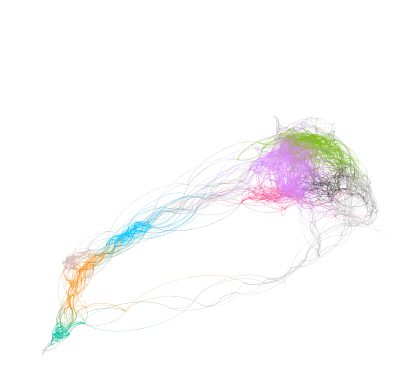
\includegraphics[width=70mm]{Figures/Results/day100-90}\label{fig:day100-90}
}
\subfloat[]{
  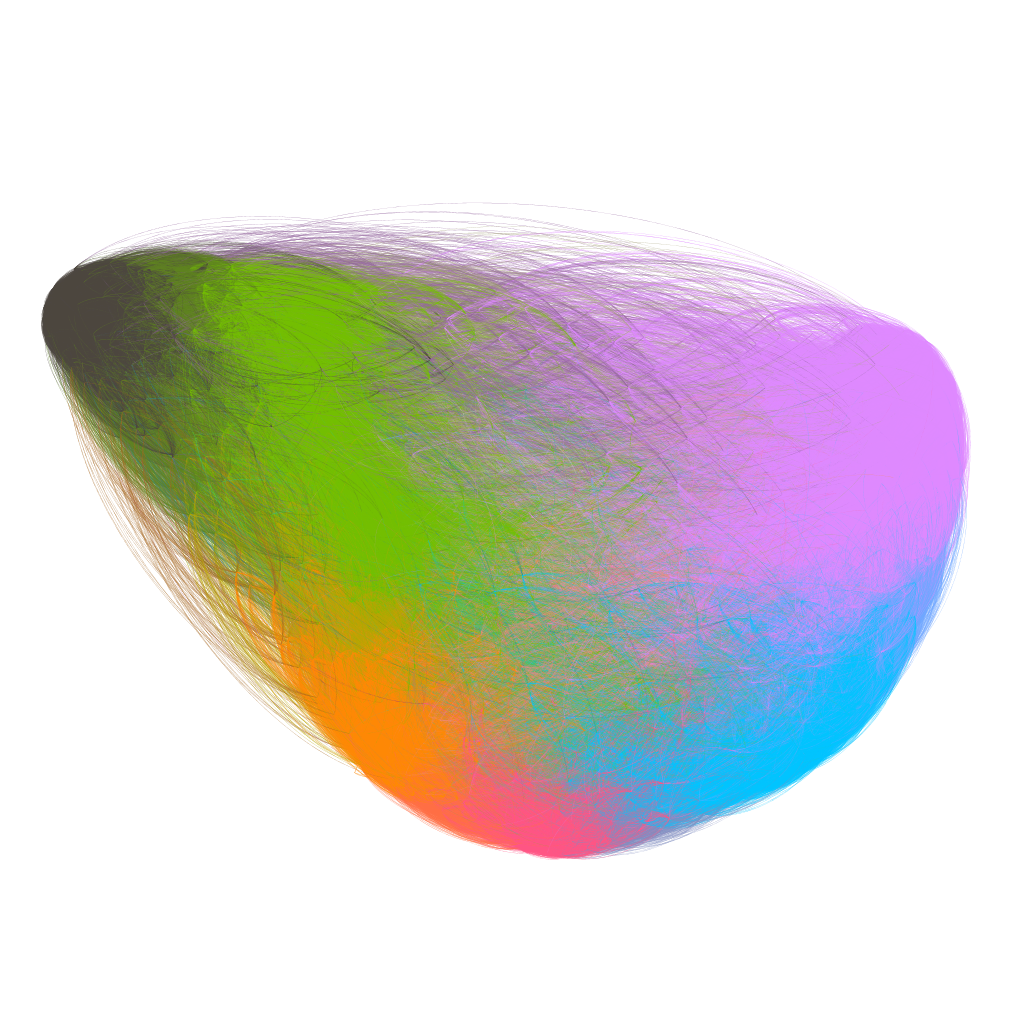
\includegraphics[width=70mm]{Figures/Results/day100-70}\label{fig:day100-70}
}

\caption[Example graphs with different cut offs]{Example of day 09-08-2011 with different correlation cut offs, nodes have been removed for ease of viewing, but edges are coloured by cluster. The difference between graphs with different cut off points can be dramatic. Figure \ref{fig:day100-90} has a cut off point of a minimum correlation of 0.9 whilst \ref{fig:day100-70} has a cut off of 0.7. As can be seen the number of edges is much higher. Clusters were detected using the Fast-Greedy algorithm.}
\label{fig:cutoff70vs90}
\end{figure*}


\section{Labelling clusters}
\label{sec:labelling}
Once all the day graphs had been made and the day labels assigned there were over 2000 total clusters. In order to get an overview of cluster behaviour the total number of clusters each day were plotted in figure \ref{fig:Total_Clusters}. The figure shows that the rolling mean number of clusters stays more or less stable at the total mean of 25.5 for all clusters and 9.4 for the large clusters. However the standard deviation is relatively large at 7.3 for the total clusters and 2.4 for the large clusters, what's more the standard deviation increases towards the end of the period, although this could be due to the onset of winter which tends to increase behaviour variation in energy use (as shown in figure \ref{fig:DailyConsumption}). In order to get a more detailed view of the behaviour of clusters a simple labelling regime was used by ranking each cluster in order of size and assigning a label to each cluster according to rank that day. This method produced figure \ref{fig:clustrank}, which shows high levels of variation from period to period in clusters of the same rank. This is understandable in the context of the the previous figure as intuitively as the number of clusters vary the size of the clusters will also vary with some inverse relation as the total number of available nodes stays constant.

\begin{figure*}[ht]
\centering
\subfloat[]{
  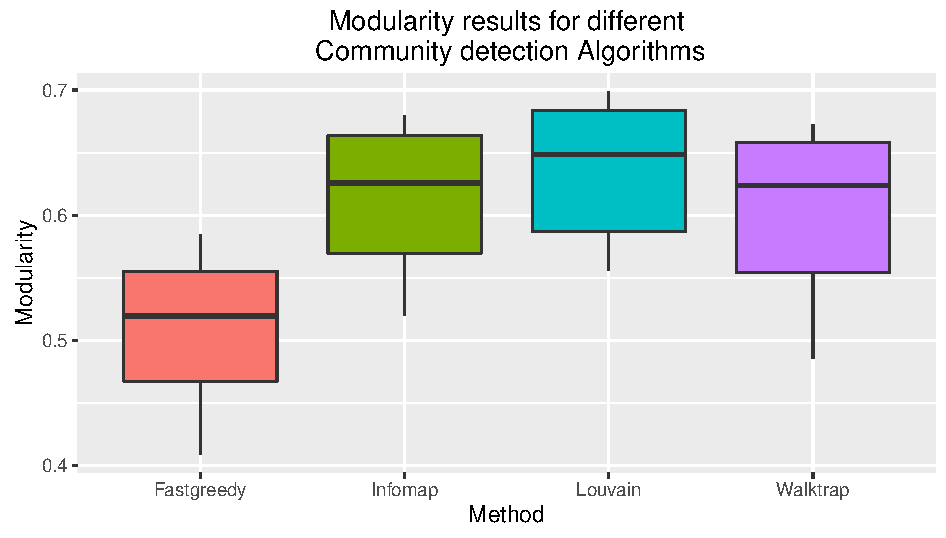
\includegraphics[width=0.80\textwidth]{Figures/Results/CommModComp}\label{fig:CommModComp}
}

\subfloat[]{
  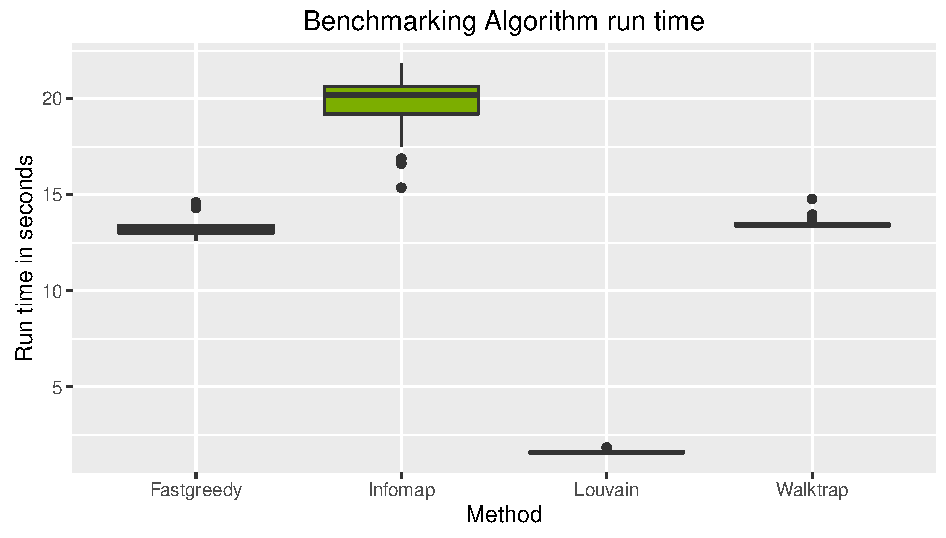
\includegraphics[width=0.80\textwidth]{Figures/Results/AlgorithmTimes}\label{fig:Algtime}
}

\caption[Cluster Family Load Profiles]{ Benchmarking the four target algorithms, shows that Walktrap, Infomap, and Louvain are all statistically similar in performance with Louvain getting slightly better results, however Louvain is considerably faster when it comes to detecting clusters}
\label{fig:ChooseAlg}
\end{figure*}



\begin{figure}[ht]
    \centering
    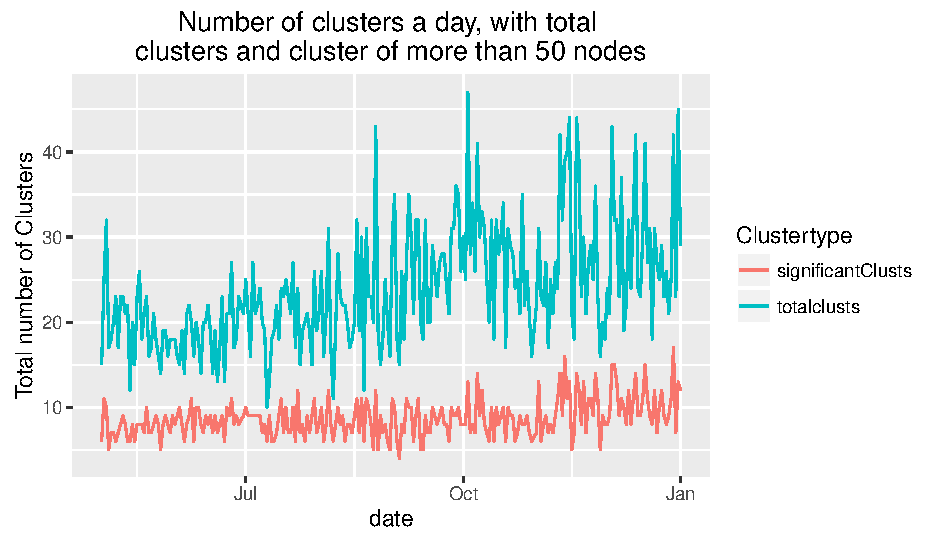
\includegraphics[width=\textwidth]{Figures/Results/TotalClusters}
    \caption[Total clusters over time]{The total number of clusters or communities detected over time has quite a large amount of variation. Although it can be seen that there are many clusters that are insignificant even the significant clusters have quite large variation }
    \label{fig:Total_Clusters}
\end{figure}

\begin{figure}[ht]
    \centering
    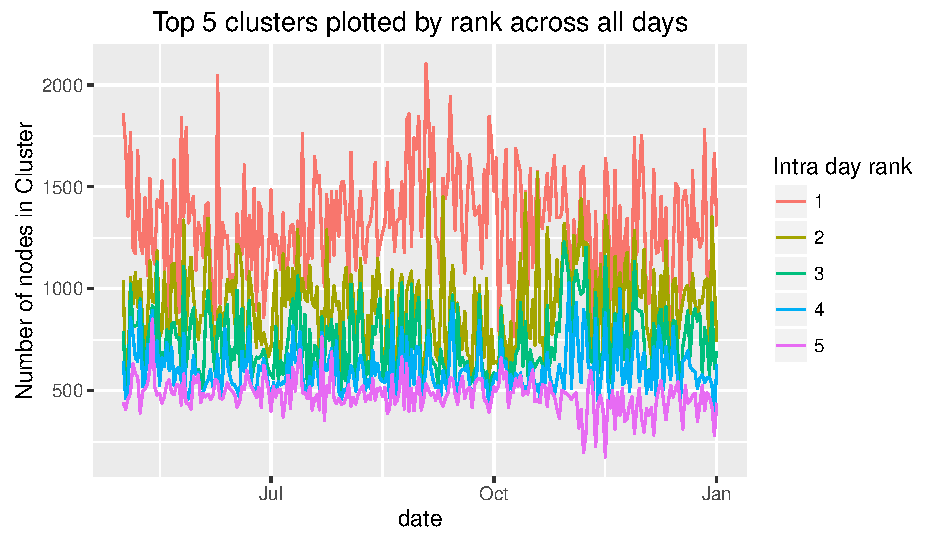
\includegraphics[width=\textwidth]{Figures/Results/Clusterrank}
    \caption[Size comparison of the largest clusters]{The total number of nodes in each cluster larger than 50. The cluster ID's are assigned by size rank. The results are interesting as there is a large amount of noise in the cluster sizes which do not hold steady throughout the period.}
    \label{fig:clustrank}
\end{figure}
\FloatBarrier 

Using the labelling method described in \ref{sec:labelClust}, the inter-cluster correlation matrix was created using clusters that had a at least 50 nodes (see fig \ref{fig:corheat}). This was then turned into a graph and communities detected using the same method as for the original graphs and community detection, but with a cut off of 0.85 instead of 0.7 as there was much more consistency in the cluster correlations. The resulting graph and communities can be seen in figure \ref{fig:DragonPlot}. These clusters can be classified into time periods as shown in \ref{fig:Familypattern}. The soup family of clusters is for clusters that are either less than 50 nodes and so are not large enough to give reasonable results, or are a cluster that is less than 1\% of the total volume of nodes in the whole 246 day period. An interesting effect on \ref{fig:DragonPlot} is that the clusters are mostly connected only within cluster and between temporarily adjacent clusters. This is because they are inherently more highly correlated with nearby clusters than ones that are further away. The clusters at the later part of the evening, specifically the 2000 and 2100 clusters, can be seen to be made up of a group of subclusters which is seen by the bumpiness in figure \ref{fig:DragonPlot}. It can also be seen more explicitly in \ref{fig:ClusterFamilySample} where both cluster 1600 and 2100 can be seen to have two peaks, whilst the 1800 cluster has got variance but had only a single peak. Figure \ref{fig:AllNodesClustercolour} in the appendix shows the compound plots of the clusters that make up each cluster family, Figure \ref{fig:AllCLustFamilies} plots all the clusters showing the separation of each cluster and the areas of overlap.

The final clusters were 1630, 1700, 1730, 1800, 1830, 1900, 2000, and the node Soup. Figure \ref{fig:Familypattern} shows how consistent these forms are using mean, median, and sum although the form breaks down somewhat on the plot of standard deviation.


\iffalse
A more consistent method of assigning labels is to use Jaccard similarity. This was calculated using the vector of nodes in each cluster as the similarity measure, this then allowed a new graph to be made and communities within that to be detected. Figure xxx shows that there is very high similarity within clusters and very low levels of similarity between clusters, suggesting that there is very little overlap between clusters in terms of nodes and that nodes seldom move between different cluster groups. One of the things that is important to consider when using Jaccard clustering is that it will create communities based on which smart meter is in each cluster not on how electricity is being consumed.
\fi

\begin{figure}[ht]
    \centering
    \textbf{Relationship between cluster families}\par\medskip
    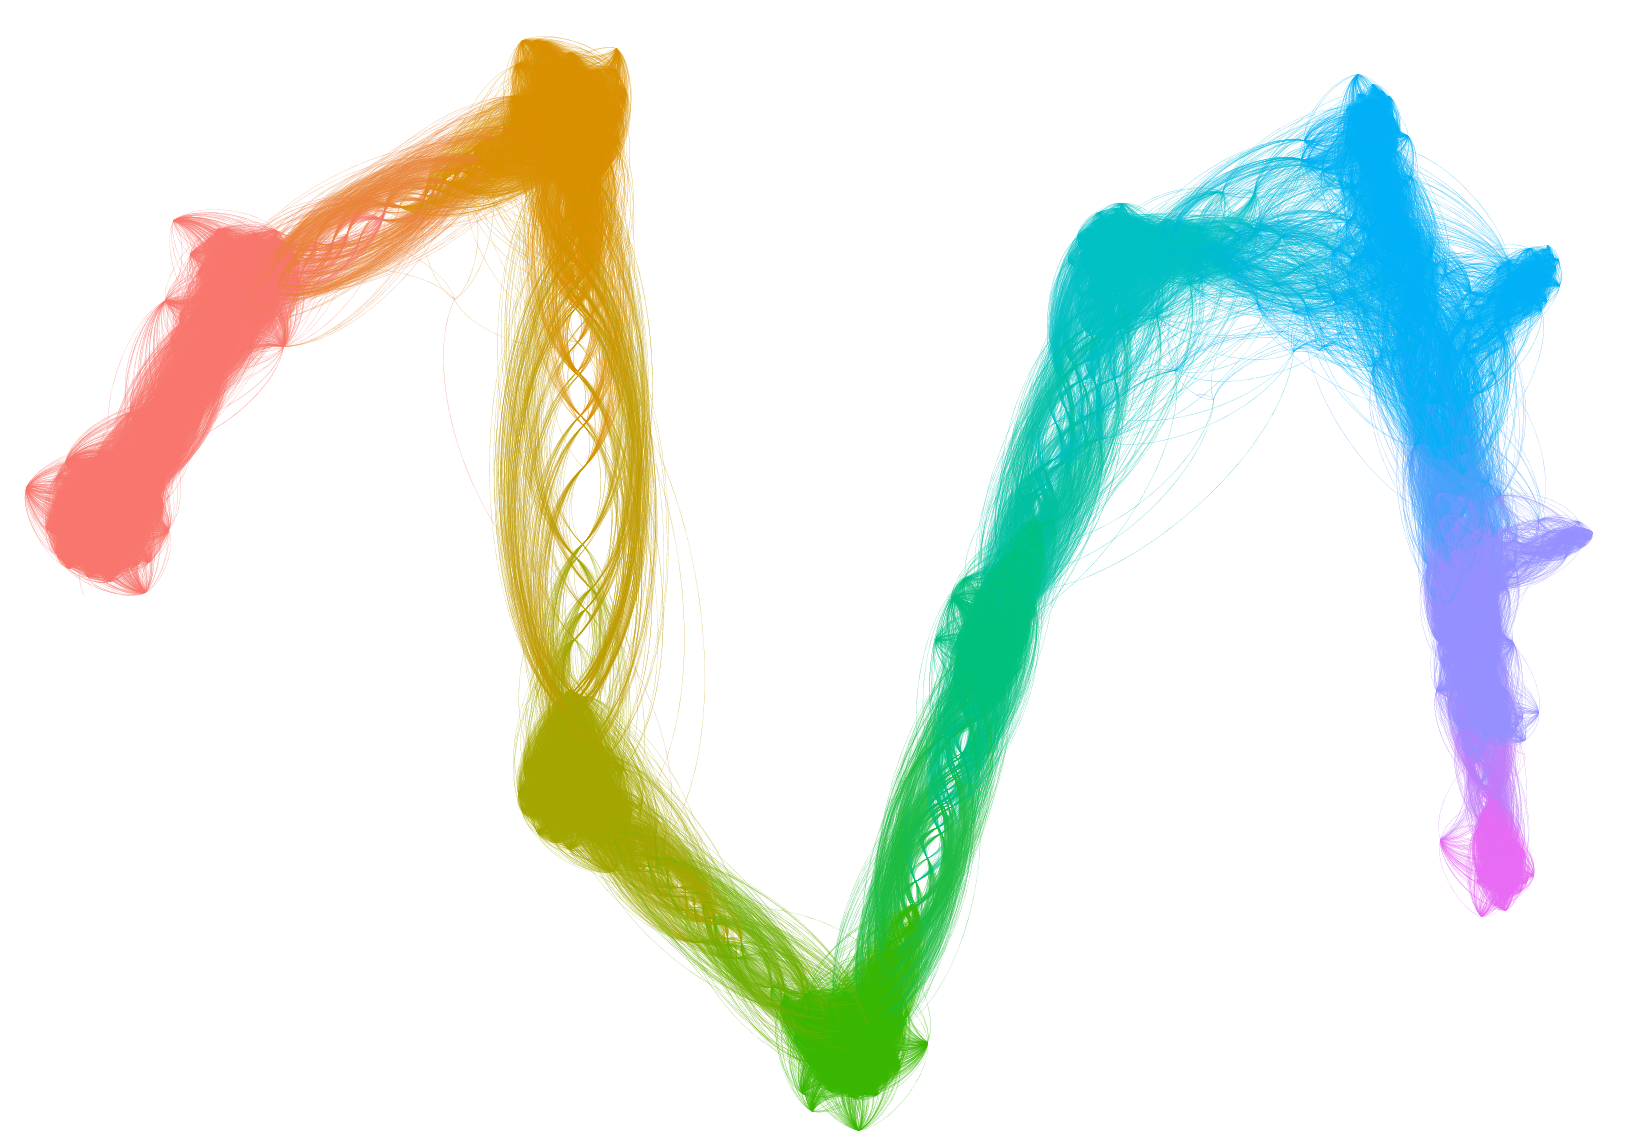
\includegraphics[width=\textwidth]{Figures/Results/Dragon}
    \caption[Cluster family Graph]{The Clusters were grouped into cluster families, each family represented a peak at a specific time of the evening, the figure shows these families, moving from the 1600 cluster on the left to the 2130 cluster on the right.}
    \label{fig:DragonPlot}
\end{figure}


\begin{figure*}[ht]
\centering
\subfloat[]{
  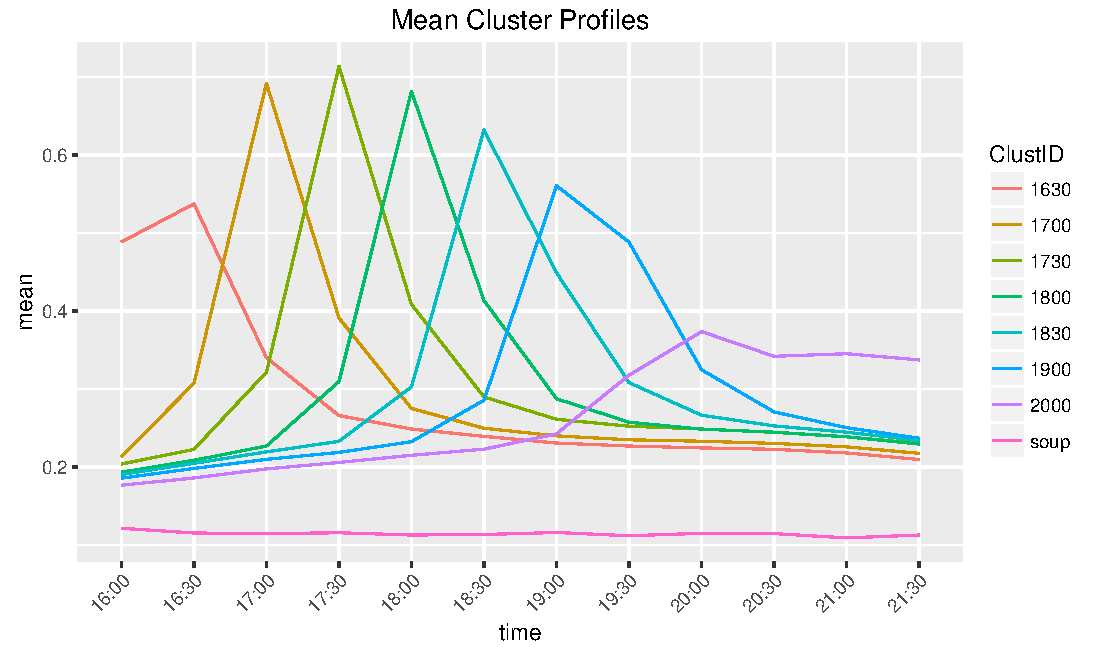
\includegraphics[width=0.49\textwidth]{Figures/Results/ProfileMean}\label{fig:Clusmean}
}
\subfloat[]{
  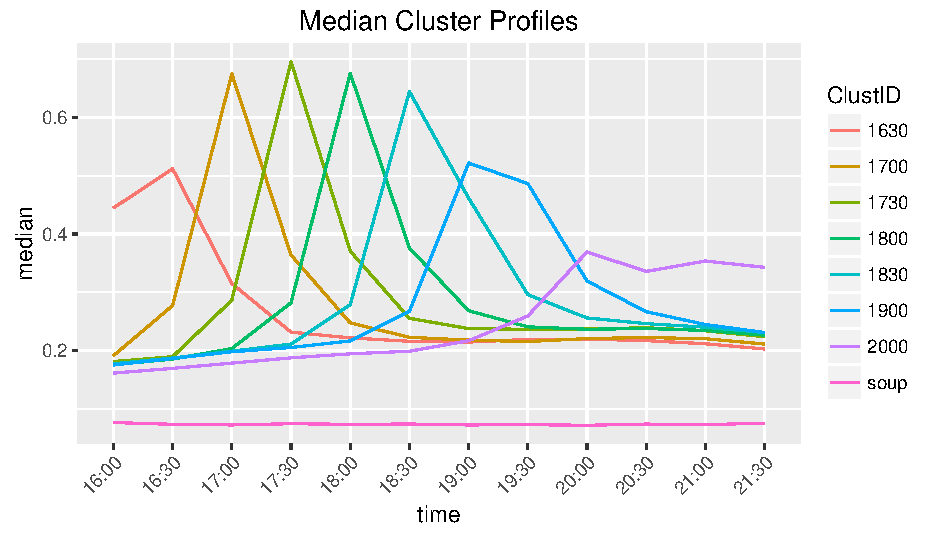
\includegraphics[width=0.49\textwidth]{Figures/Results/ProfileMedian}\label{fig:Clusmedian}
}

\subfloat[]{
  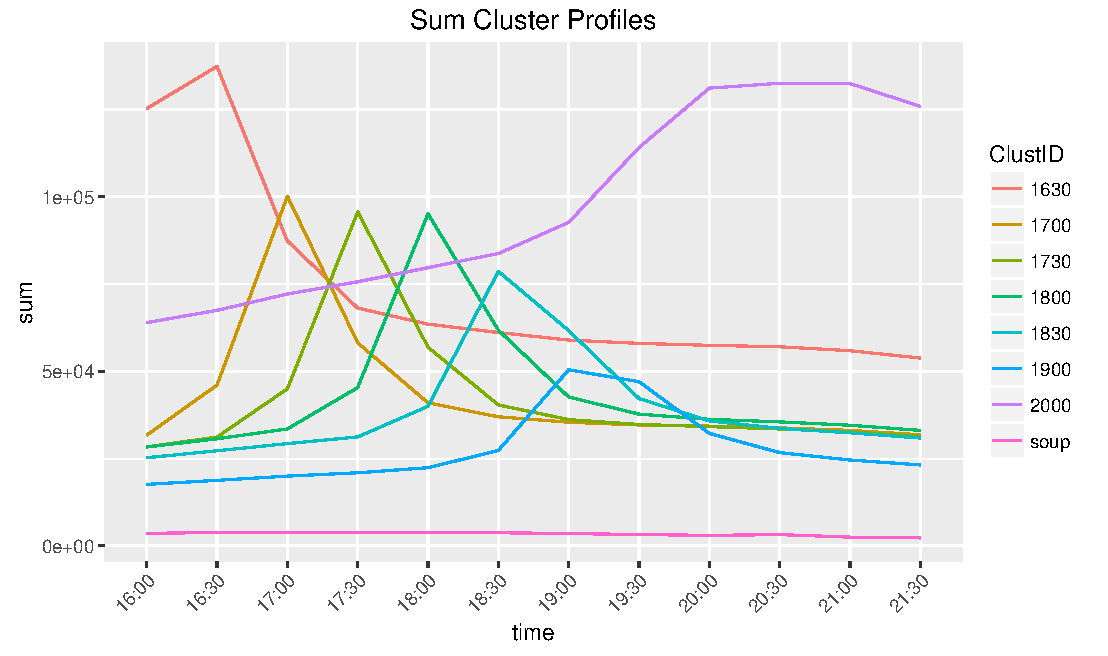
\includegraphics[width=0.49\textwidth]{Figures/Results/ProfileSum}\label{fig:CLussum}
}
\subfloat[]{
 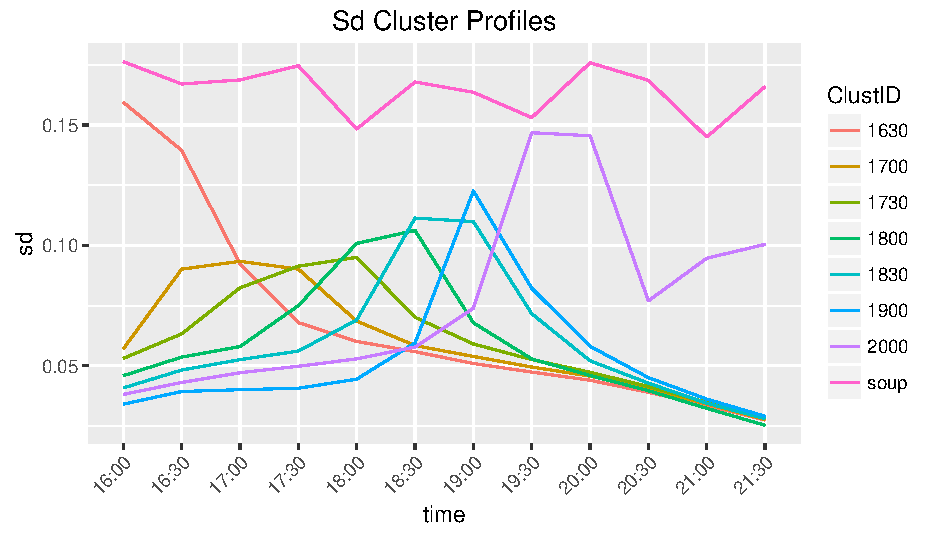
\includegraphics[width=0.49\textwidth]{Figures/Results/ProfileSd}\label{fig:Clusvar}
}
\caption[Cluster Family Load Profiles]{This series of figures is similar to \ref{fig:daypattern}, except instead of showing the day load profile, it shows the load profile for the cluster families overall. As can be seen in \ref{fig:Clusvar} variance is considerably lower than in \ref{fig:dayvar}, this is because the clustering causes an information loss smoothing the final result and reducing aggregate results.}
\label{fig:Familypattern}
\end{figure*}


\begin{figure}[ht]
    \centering
    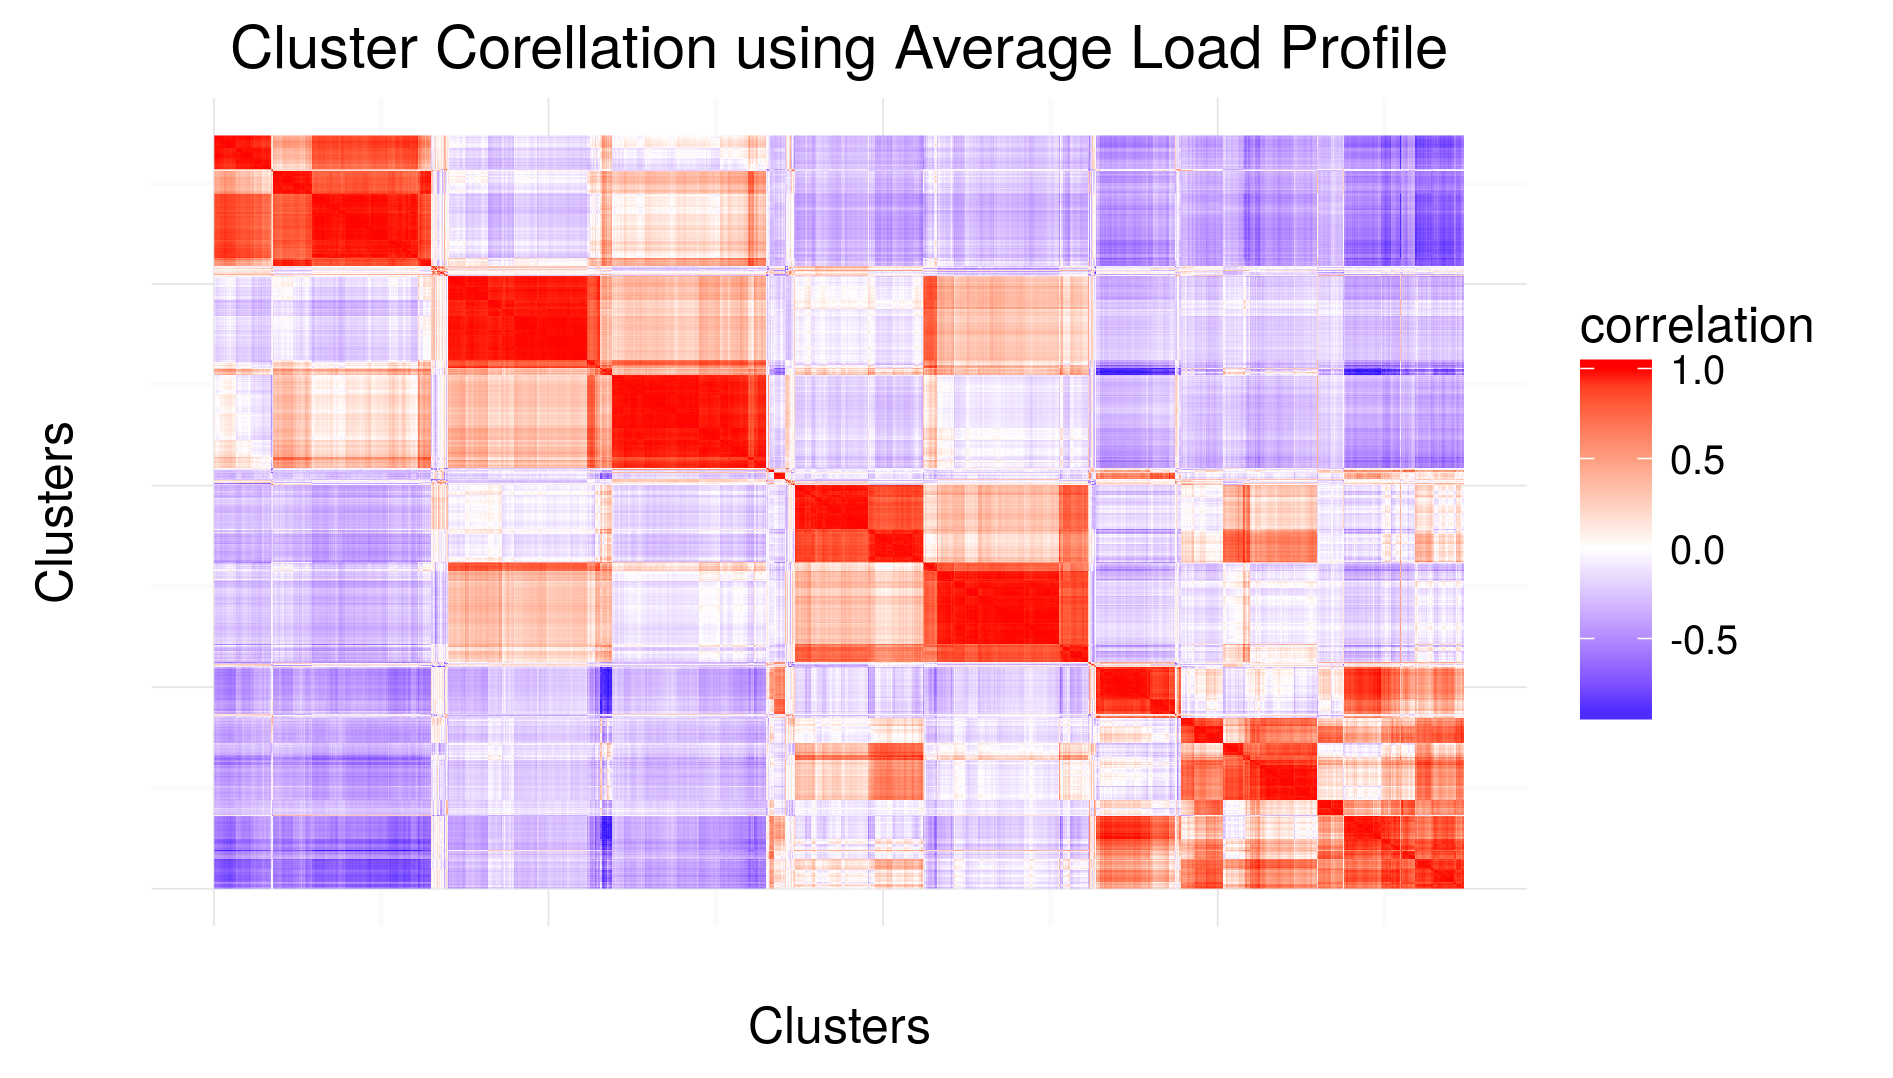
\includegraphics[width=\textwidth]{Figures/Results/ClusterCorLoadLarge.png}
    \caption[Cluster similarity heatmap]{The heat map of Cluster similarity shows that there are very low levels of cross cluster similarity and very high levels of within cluster similarity. The modularity of these communities was 0.83}
    \label{fig:corheat}
\end{figure}

\begin{figure}
    \centering
    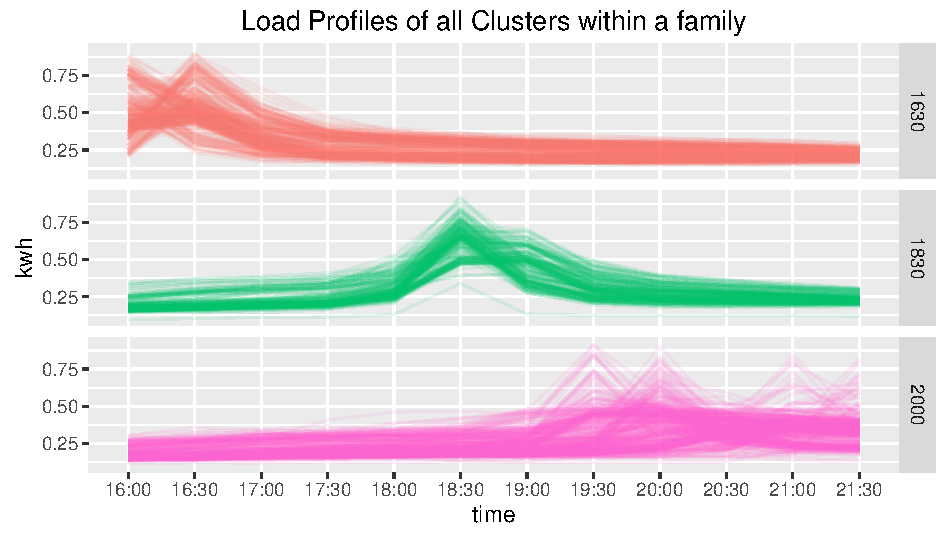
\includegraphics[width=\textwidth]{Figures/Results/ClusterFamilySample}
    \caption[Within Cluster Family Node Profile]{The figure shows all the clusters from the same family layered on the same plot.}
    \label{fig:ClusterFamilySample}
\end{figure}


After the cluster families had been decided, it was important to see how frequently each of the cluster families occurred across the time period. Figure \ref{fig:Clusterocurrance} shows red if the cluster is present and blue if the cluster is not present. Only cluster 1630 is present on all days cluster 1700, 2000 and the soup are present on most days, the 1900 cluster can be especially sparse a fact that causes prediction problems in \ref{fig:BoxTimeErr}. It's interesting consider that the node soup does not occur everyday, this means that on some days there are no nodes with significantly different behaviours. Missing clusters is most likely a side effect of using non-overlapping clustering algorithms and hard clustering nodes into only 1 cluster. 
Figure \ref{fig:SankeyWeek} shows a Sankey or Alluvial diagram \cite{sankeydiagrams} \cite{rosvall2010} which visualises flow and thus can be used to represent change in network structure. The Sankey diagram shows the volume of flow between clusters across days and it is possible to see days when clusters are missing in this case day 4 (07-08-2011) is missing the 1730 cluster. As can be seen the clusters all transition to each other to some degree, this makes the sudden disappearance of a cluster seem and unrealistic reflection of behaviour patterns and more an artifact of the clustering process. Looking at the Sankey diagram it can seem like the transitions are simply proportional to the size of the cluster however the $\chi ^2$ test of the transition matrix and node distribution in \hl{XXX} show that there is in fact a structure to the movement.

\begin{figure}
    \centering
    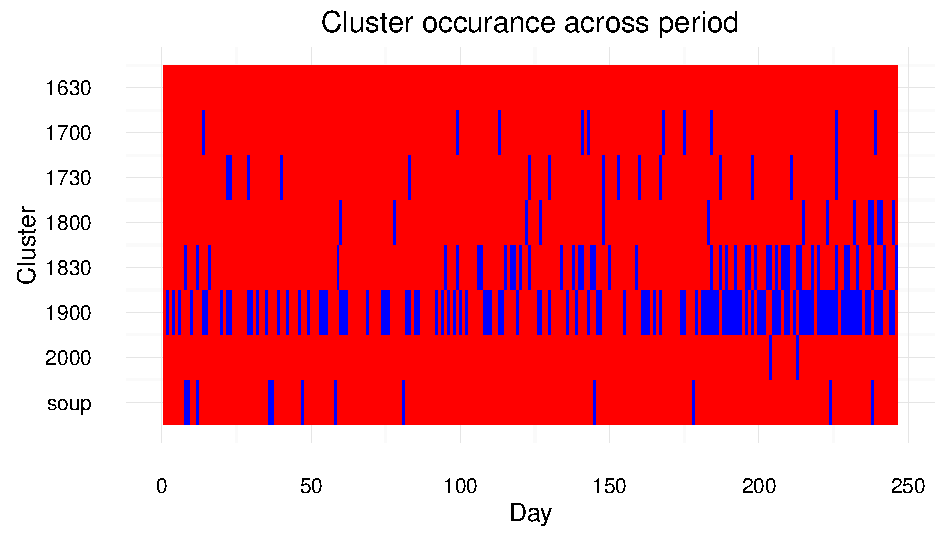
\includegraphics[width=\textwidth]{Figures/Results/Clusterocurrance}
    \caption[Cluster Occurance]{The occurrence of each cluster family across all days. As each node is clustered exclusively into a single cluster each day, it can happen that some days not all clusters are present. This doesn't mean that there were no nodes peaking at that time but is more an artifact of using non-overlapping clustering algorithms.}
    \label{fig:Clusterocurrance}
\end{figure}


\begin{figure}[ht]
    \centering
    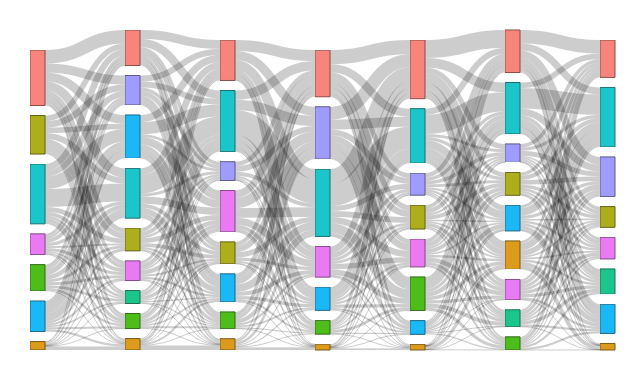
\includegraphics[width=\textwidth]{Figures/Results/SankeyWeek.png}
    \caption[Sankey diagram for 1 week]{Sankey Diagram showing the week including Saturday 09-08-2011 which is the $6^{th}$ day/layer of the Sankey Diagram, the colour scheme is the consistent with the Cluster labels elsewhere in this work, e.g the node soup shown in red. The order of the clusters in each day are optimised to reduce cross over, however as can be seen there is a lot of cross cluster movement of nodes between days, this reflect the probability of transfer seen in the transition matrix. }
    \label{fig:SankeyWeek}
\end{figure}


\subsection{Looking at cluster load profiles for a single day}

As a control, looking at an individual days load profile is instructive. Using 09-08-2011 as an example figure \ref{fig:daypattern} shows the load profiles of each cluster, table \ref{table:NodesPerCluster}, gives the nodes per cluster. The figure shows that each cluster exhibits a clear and distinct load profile across each metric similar to the cluster families in figure \ref{fig:Familypattern}. What is surprising is that the standard deviation of the profiles also reflects the over all profile pattern, to a much higher degree than in the plot of the cluster families, This is because the smoothing effect of the clustering has not been applied and so there is more natural variation possible than in the aggregated values of the clusters.

\begin{figure*}[ht]
\centering
\textbf{Day Load Profiles for 09-08-2011}\par\medskip
\subfloat[]{
  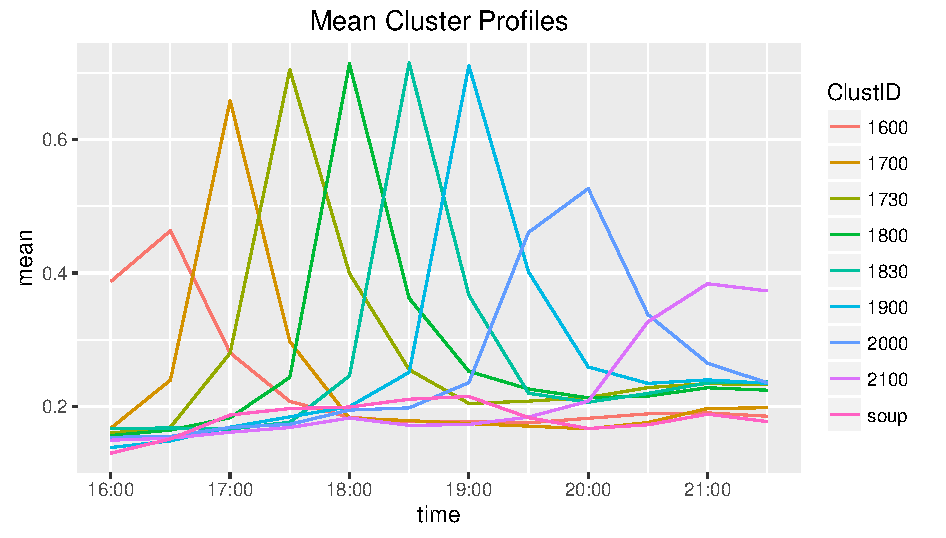
\includegraphics[width=0.49\textwidth]{Figures/Results/singledaypatternMean}\label{fig:daymean}
}
\subfloat[]{
  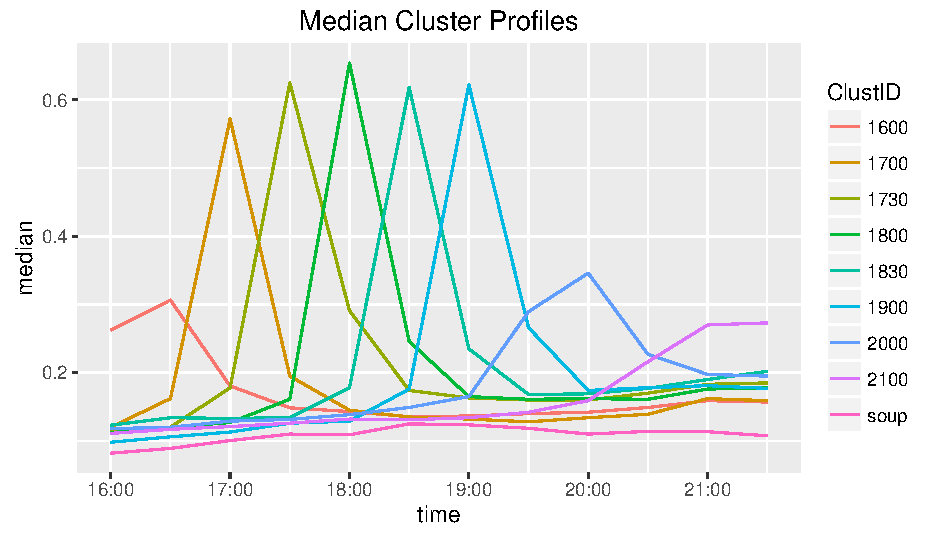
\includegraphics[width=0.49\textwidth]{Figures/Results/singledaypatternMedian}\label{fig:daymedian}
}

\subfloat[]{
  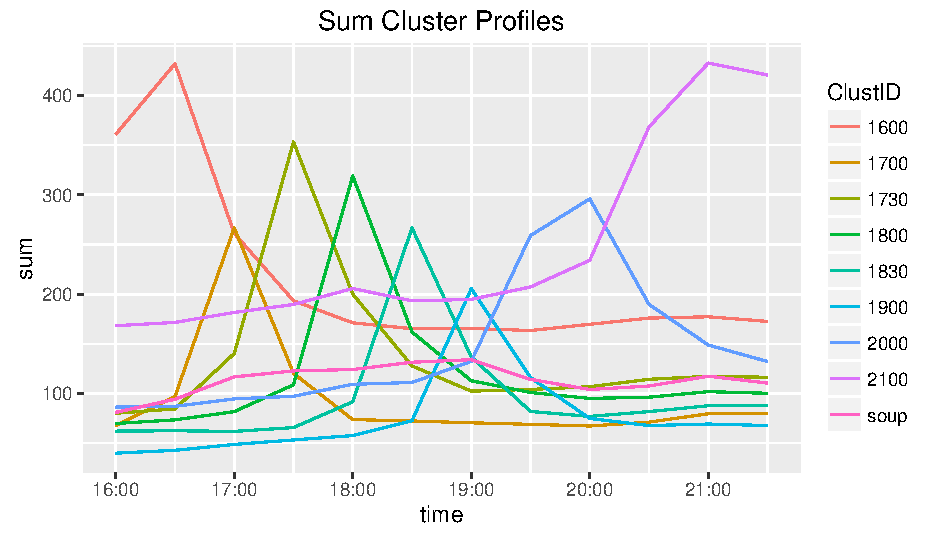
\includegraphics[width=0.49\textwidth]{Figures/Results/singledaypatternSum}\label{fig:daysum}
}
\subfloat[]{
 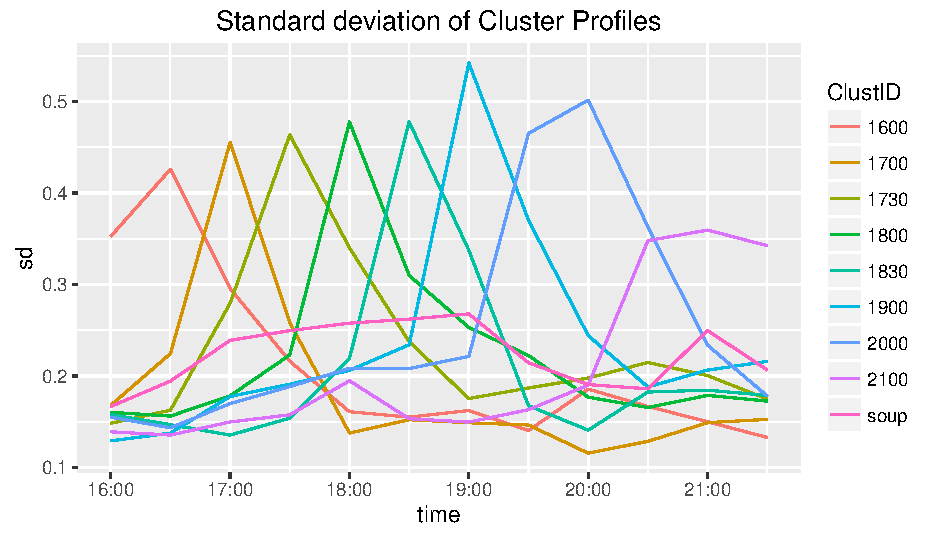
\includegraphics[width=0.49\textwidth]{Figures/Results/singledaypatternVar}\label{fig:dayvar}
}
\caption[Day Load Profiles for 09-08-2011]{This series of figures shows the pattern for day 09-08-2011 with a .7 cut off using walktrap clustering}
\label{fig:daypattern}
\end{figure*}


% latex table generated in R 3.3.0 by xtable 1.8-2 package
% Wed Aug 17 16:14:55 2016
\begin{table}[ht]
\centering
\begin{tabular}{rlr}
  \hline
 & ClustID & count \\ 
  \hline
1 & 1630 & 946 \\ 
  2 & 1700 & 508 \\ 
  3 & 1730 & 546 \\ 
  4 & 1800 & 520 \\ 
  5 & 1830 & 406 \\ 
  6 & 1900 & 657 \\ 
  7 & 2000 & 1604 \\ 
  8 & soup &  73 \\ 
   \hline
\end{tabular}
\caption[Nodes per cluster]{The total number of nodes in in each cluster for 09-08-2011} 
\label{table:NodesPerCluster}
\end{table}



\begin{figure}
    \centering
    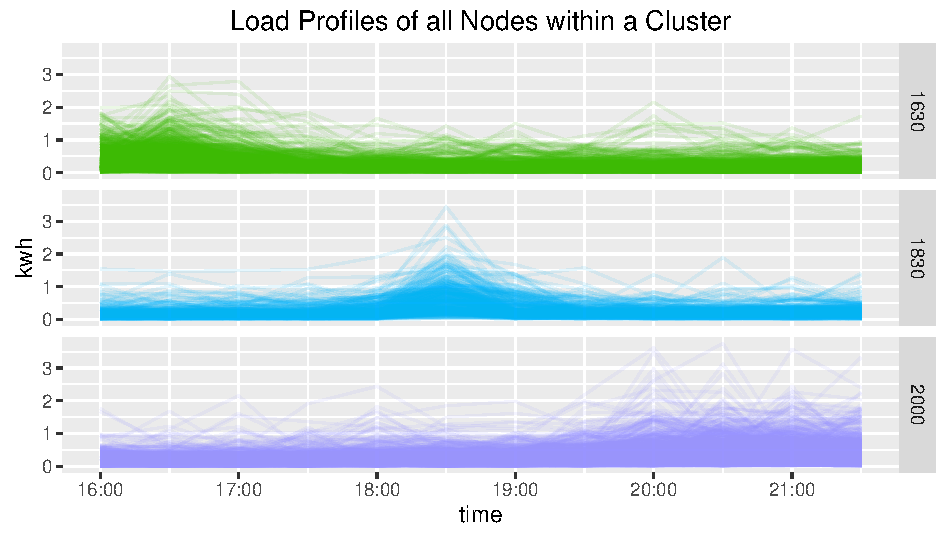
\includegraphics[width=\textwidth]{Figures/Results/NodeProfilesInCluster}
    \caption[Within Cluster Node Profile]{The within Cluster Node Profile show that although there is a lot of noise the nodes generally have their peaks at similar times. It is worth remembering that the edges and weights were decided by using a Spearman correlation which takes the rank similarity not the similarity itself.}
    \label{fig:NodeProfilesInCluster}
\end{figure}


\section{Analysing probability distributions}

After the clusters had been divided into families and their behaviour classified it was interesting to explore how the clusters and nodes interacted. Figure \ref{fig:TransitionHeat} shows a heat map of the transition matrix (the table of probabilities can be seen in \ref{tab:clustrans}). This heat map shows the probability of a node transitioning from cluster A to cluster B on consecutive days. Although there is no extremely high probability of transfer on the table it can be seen that there is a higher probability of transitioning to the same cluster than other clusters. Cluster 1600 and cluster 2100 have the highest probability of being transferred to from other clusters. 
Along with the Soup, clusters 1600 and 2100, also have the highest probability that nodes will stay within the cluster across days and not transfer out.
These insights are interesting as it implies that certain nodes consistently follow patterns that are not in any of the main clusters and so are more likely to remain in the soup. Also that people tend towards the 1600 and 2100 nodes despite the fact that they are at different ends of the evening. It's interesting to reflect why the 1600 and 2100 nodes are so popular, 
One reason may be that in the UK schools finish at 1530 and so the 1600 cluster reflects the time that children get home, in this circumstance it there would be a large group of people who would usually get back at the same time. This would explain the higher transfer probability and also the relatively large size of the 1600 group. The 2100 group could be professionals without children who have been working late or have spent the early part of the evening out before returning home. An alternative idea for the 2100 group is that it is an artifact of the simplifying of the clustering process and that people are active at other parts of the evening but that this time is peak TV watching and so many people are being clustered there due to television watching habits.


\begin{figure}[ht]
    \centering
    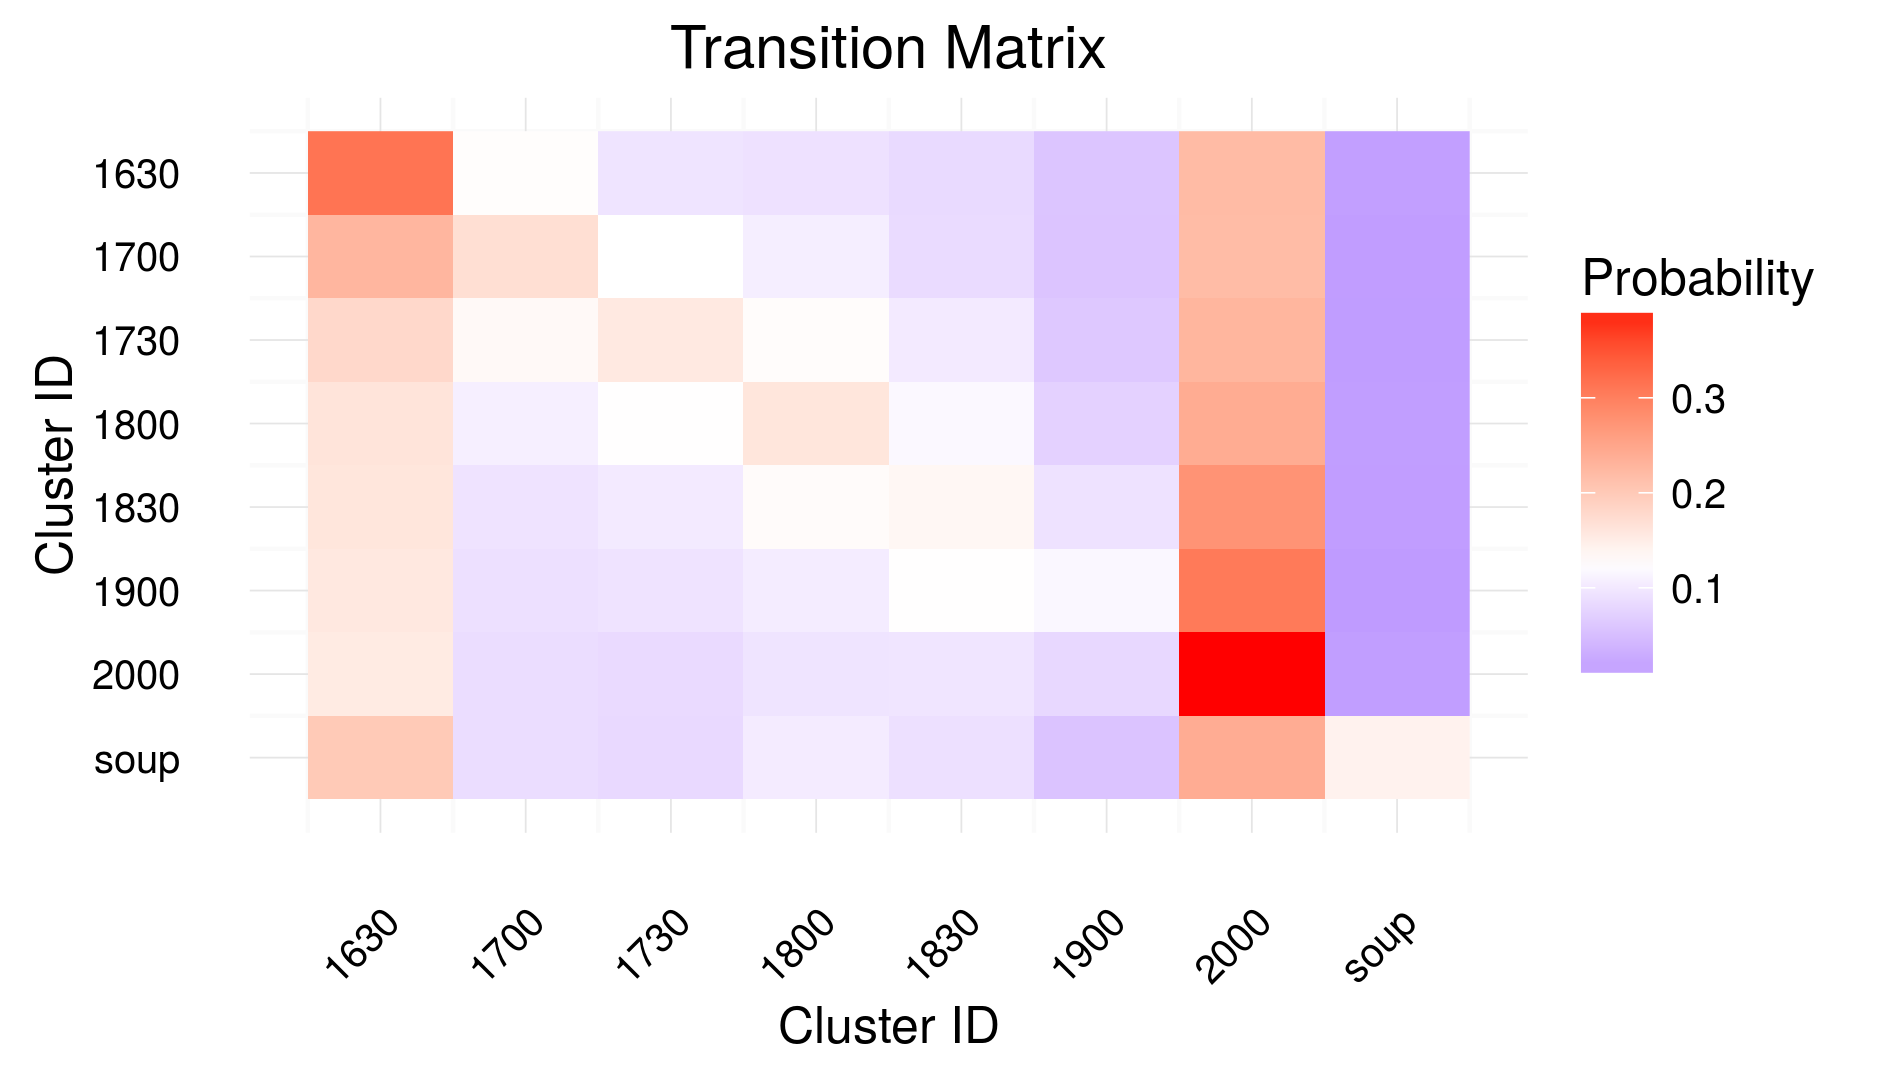
\includegraphics{Figures/Results/Clusttransgraph.png}
    \caption[Cluster family transition matrix]{The heatmap of the transition matrix makes cross cluster transition easier to understand, higher probability of transitioning is in red and low is in blue. Nodes in clusters 1600, 2000 and the Soup have the highest probability of of staying in the same cluster from one day to another. Clusters 1600 and 2000 are most likely to be transitioned too from other clusters across days.}
    \label{fig:TransitionHeat}
\end{figure}


Looking at the entropy measure Figure \ref{fig:stabilitydens} shows that the nodes have relatively high entropy and that it is strongly left skewed, this indicates that the majority of the nodes move around a lot whilst a small number are very stable. The mean value of the entropy is 1.71 the entropy which is lower than the entropy of the cluster distribution as a whole which is 1.88, again this indicates that there is structure in the distribution of nodes across clusters. Another way to look at the transfer of nodes between clusters is to look at the flow of clusters from day to day, this is shown in the Sankey diagram in figure \ref{fig:SankeyWeek}, although the diagram is noisy it is possible to see the patterns of movement reflected in the transition matrix.


\begin{figure}[ht]
    \centering
    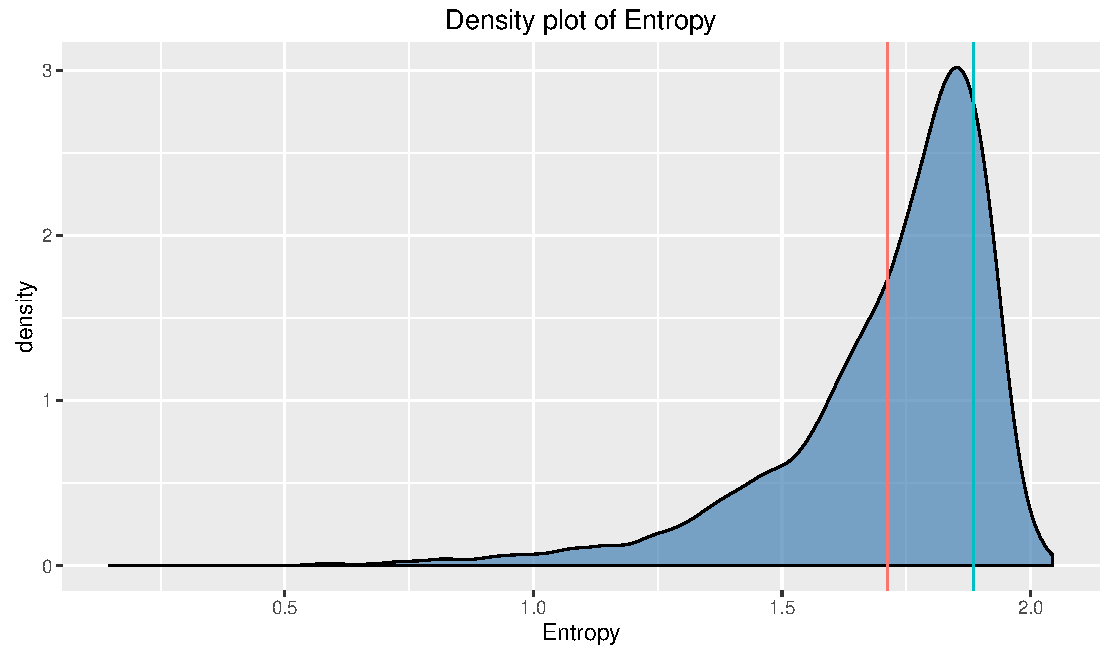
\includegraphics{Figures/Results/stabilitydens}
    \caption[Entropy density]{The plot shows the density distribution of the entropy across all nodes. The entropy of the clusters overall is shown as the red verticle line, everything to the right has less information than random.}
    \label{fig:stabilitydens}
\end{figure}


\FloatBarrier

\section{Modelling}
With the transition matrix and the bi-variate probability tables completed and tested to ensure that each table's dependencies are not random, it possible to create a forecasting model to predict day ahead portfolio load, node cluster membership and socio-demographic class. 

\subsection{Power forecasting}
The creation of a forecasting model using a transition matrix and it's comparison to a linear model baseline showed that clustering as a form of classification is an effective method for predicting day ahead domestic electricity consumption. The transition matrix was made using data from the 01-05-2011 to 15-11-2011, the test period was from 16-11-2011 to 01-01-2012.

The Transition model had an RMSE of just under 100 and a MAPE of less that 4\% this out performed the linear model which had an RMSE of 140 and a MAPE of just over 5\%, a table showing the relative performance of the two models is shown in table \ref{tab:modperf}. Figure \ref{fig:ActualVsPredLine} compares the actual to the predicted values of the model. The model tracks the actual values well but with some noise, which is most likely due to the absolute clustering caused by classifying each node into an single cluster instead of taking a more basyian probability distribution approach to cluster membership, As mentioned in figure \ref{fig:Clusterocurrance} this can result in clusters being missing on certain days and could result in artificially 'over-filling' certain clusters. The effect of missing data can be most clearly seen in the 1900 hundred cluster which is shown as a consistent outlier in \ref{fig:AbsPercErrLine} and as highly missing overall especially in the test period as shown in \ref{fig:Clusterocurrance}. 

Figures \ref{fig:resids} and \ref{fig:AbsPercErrLine} show the total error per half hour across all days and the percentage error. It can be seen that the model tends to over estimate the amount of energy in the early part of the evening until 1900 when there is an error spike of under estimation after which the bias disappears and the error varies around 0. The 1900 spike is shown in the percentage error figure to be the biggest point of error in the model when excluding outliers. The outlying day is 12-12-2011, a day with high levels of missingness that was included to ensure that the days were contiguous from the the first to the last date in the set. The missing values were imputed using the method in \ref{sec:imputation}. 
Intuitively National Holidays or days of cultural importance would have an effect on the overall domestic load. as Christmas falls in the test period it would therefore be expected that Christmas eve and Christmas day would show as outliers in the prediction model, however as figures \ref{fig:resids} and \ref{fig:AbsPercErrLine} show, these days do not in fact behave significantly differently from other days in the test period.

Figure \ref{fig:ActualVsPredErr}, is a scatter plot of half hourly predictions vs the actual load, the figure is coloured by percentage error and has the line of perfect fit shown in black. It can be seen in the figure that the model has a relatively low bias, tracking the perfect fit line well, The outlying day is shown as dark red spots above the line.

Given the low levels of error and the few strong outliers that are shown in the first 3 figures, It the density plot of the error shown in figure \ref{fig:ErrDistrib} is unsurprising. It shows a highly dense absolute error with the majority of the weight between 0\% and 5\% but that there is a long right tail indicating outliers, specifically the highly imputed 12-12-2011.

Breaking the model into half hourly performance figure \ref{fig:BoxTimeErr} shows that error across all time periods is similar with the exception of 1900 which has considerably higher than expected error as was seen in \ref{fig:resids} and \ref{fig:AbsPercErrLine}. Finally figure \ref{fig:ResidualsTime} plots a time series of the errors showing how disproportionally large the error in 12-12-2011 was, although as mentioned earlier in this section removing this day doesn't have an large effect of on the overall effectiveness of the model.

\begin{figure}
    \centering
    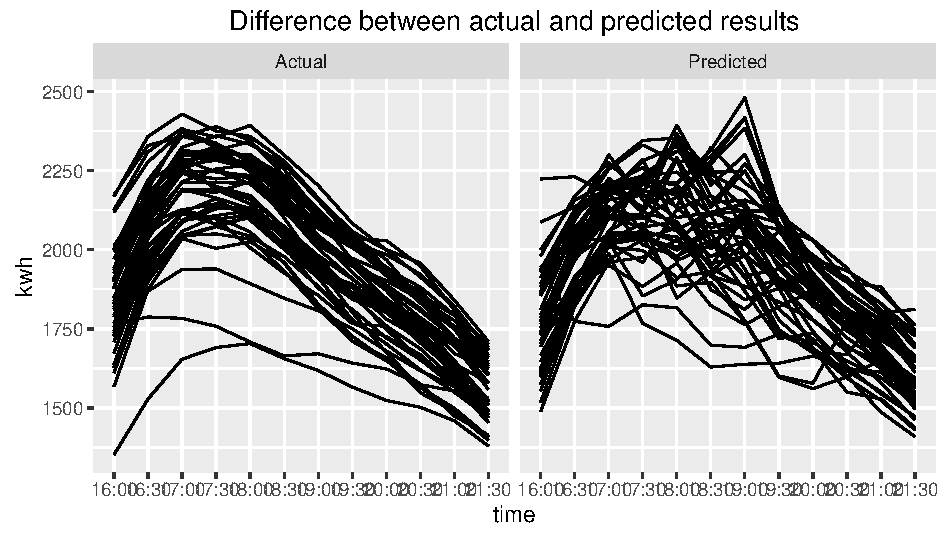
\includegraphics[width=\textwidth]{Figures/Results/ActualVsPredLine}
    \caption[Comparing actual vs predicted results]{The figure shows how the predicted values track the actual values, the general form can be seen but with noise induced. The spike of the 1900 cluster is visible as an outlier.}
    \label{fig:ActualVsPredLine}
\end{figure}

% latex table generated in R 3.3.0 by xtable 1.8-2 package
% Wed Aug 17 16:04:31 2016
\begin{table}[ht]
\centering
\begin{tabular}{rlrr}
  \hline
 & type & LinearMod & TransMod \\ 
  \hline
1 & mape & 0.05 & 0.04 \\ 
  2 & R\verb|^|2 & 0.68 & 0.84 \\ 
  3 & RMSE & 140.84 & 99.20 \\ 
   \hline
\end{tabular}
\caption{Performance metrics for the two model types} 
\label{tab:modperf}
\end{table}


\begin{figure*}[ht]
\centering
\subfloat[]{
  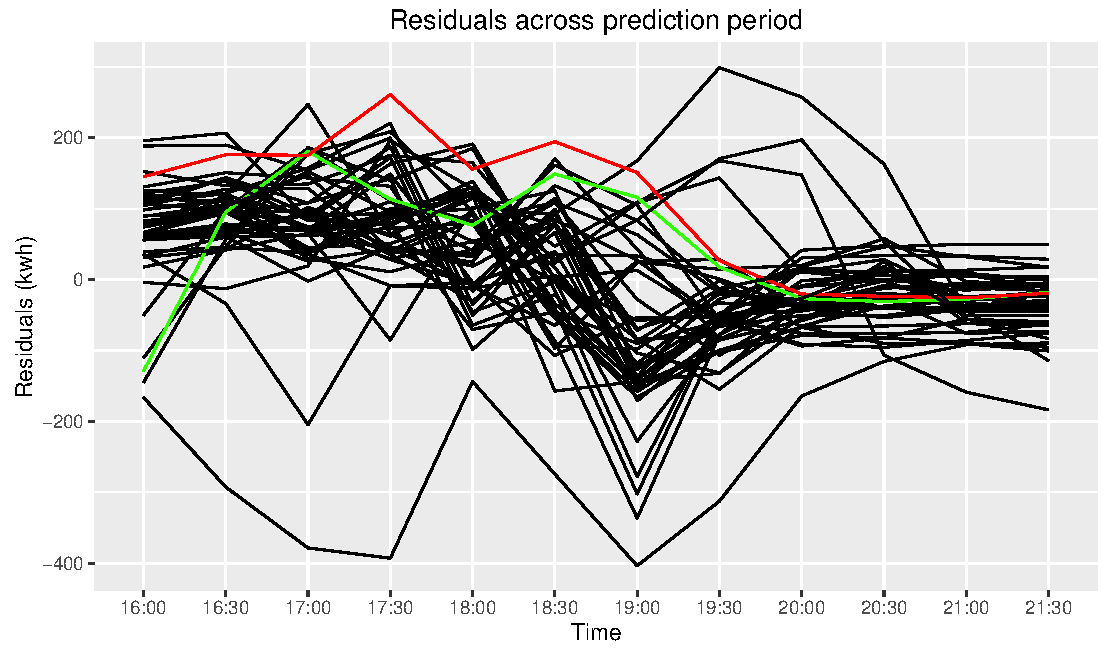
\includegraphics[width=0.49\textwidth]{Figures/Results/ResidsWXmas}\label{fig:resids}
}
\subfloat[]{
  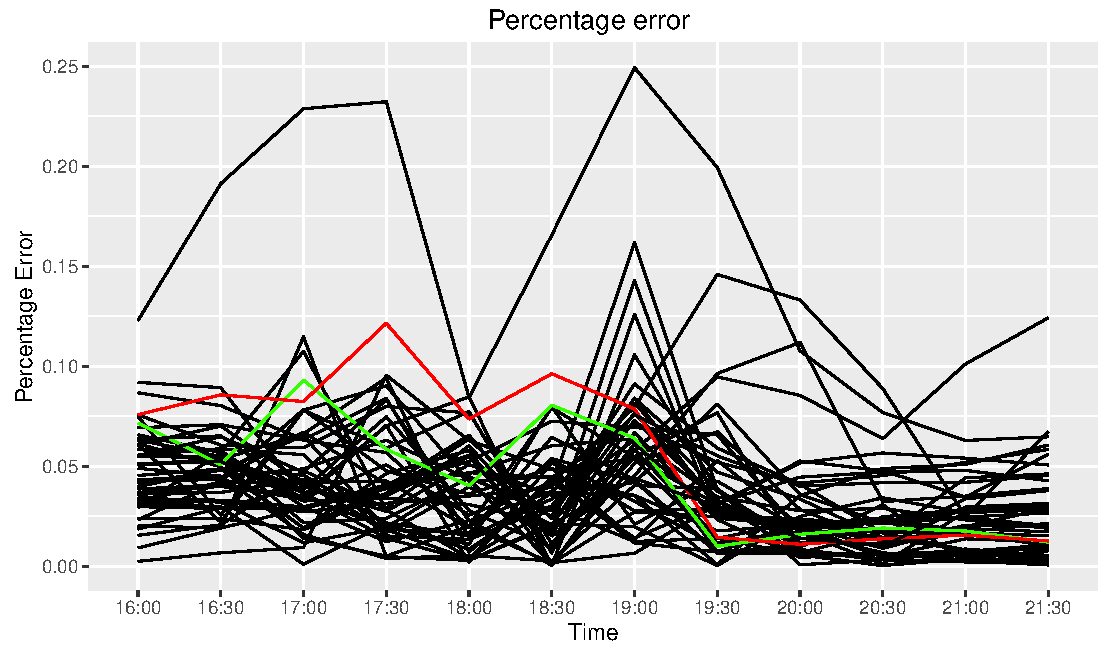
\includegraphics[width=0.49\textwidth]{Figures/Results/AbsPercErrLine}\label{fig:AbsPercErrLine}
}

\subfloat[]{
  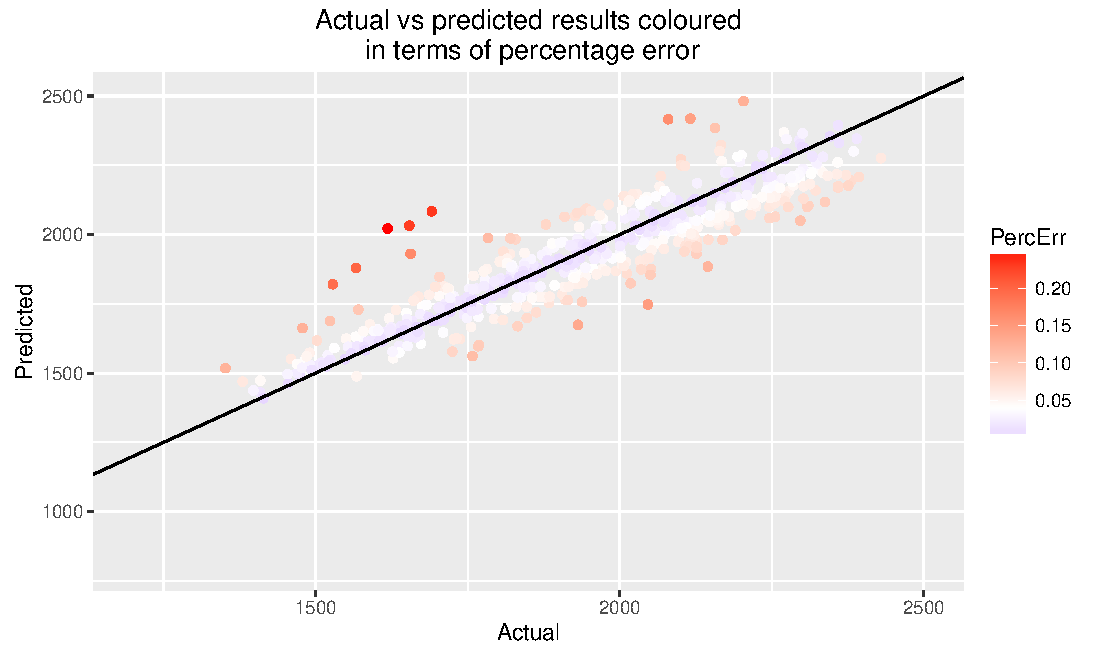
\includegraphics[width=0.49\textwidth]{Figures/Results/ActualVsPredErr}\label{fig:ActualVsPredErr}
}
\subfloat[]{
 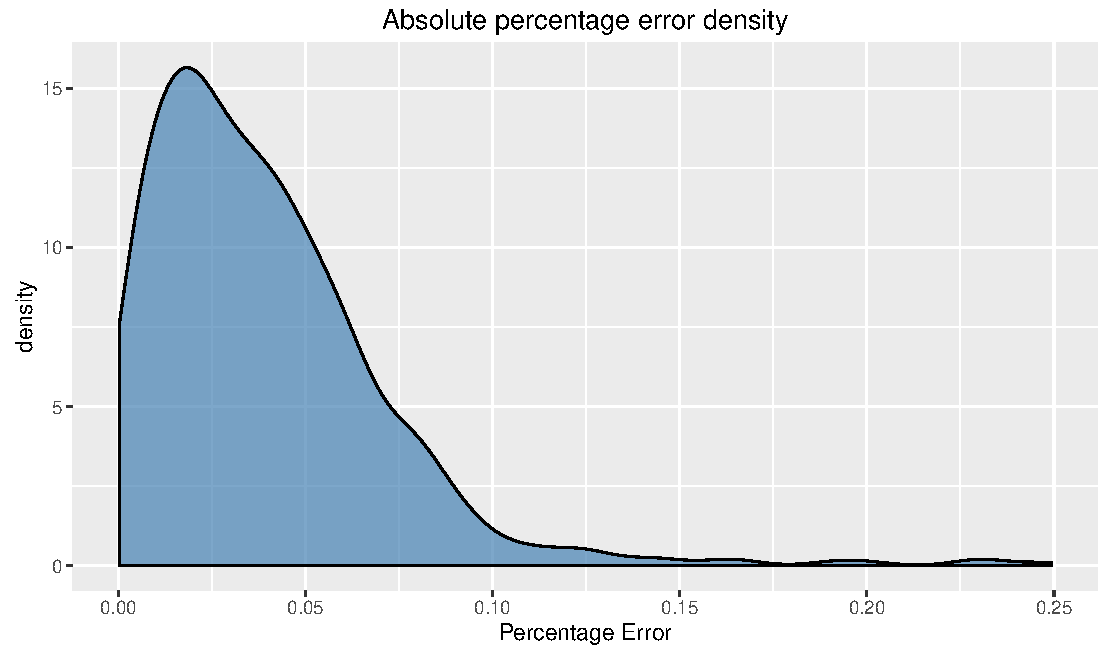
\includegraphics[width=0.49\textwidth]{Figures/Results/AbsPercErrDistrib}\label{fig:ErrDistrib}
}

\subfloat[]{
  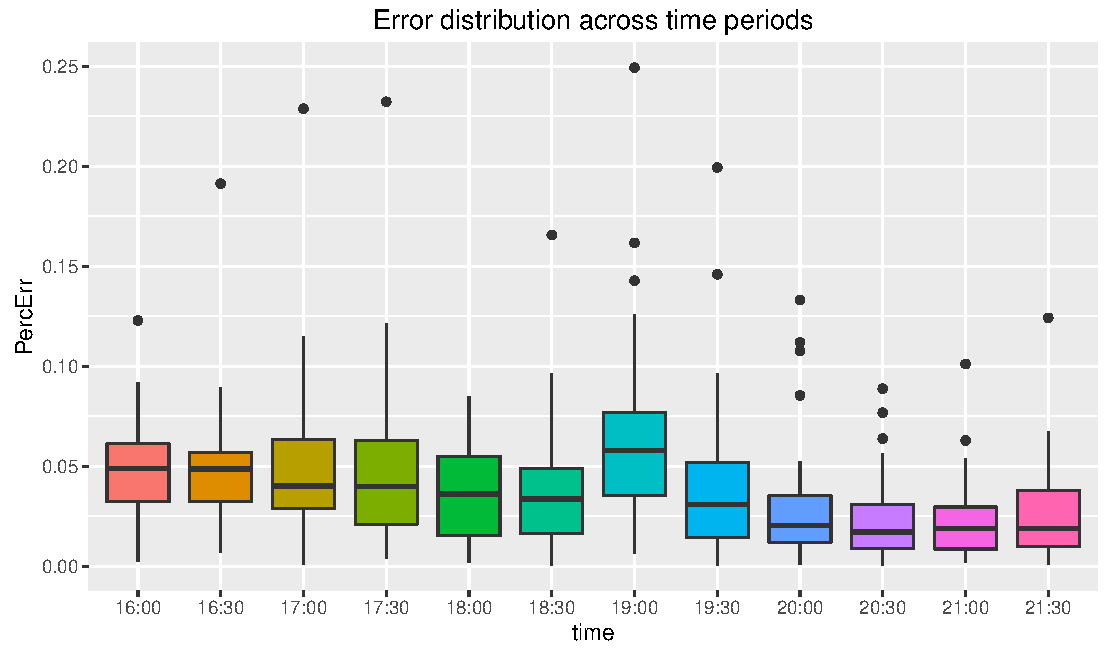
\includegraphics[width=0.49\textwidth]{Figures/Results/BoxTimeErr}\label{fig:BoxTimeErr}
}
\subfloat[]{
 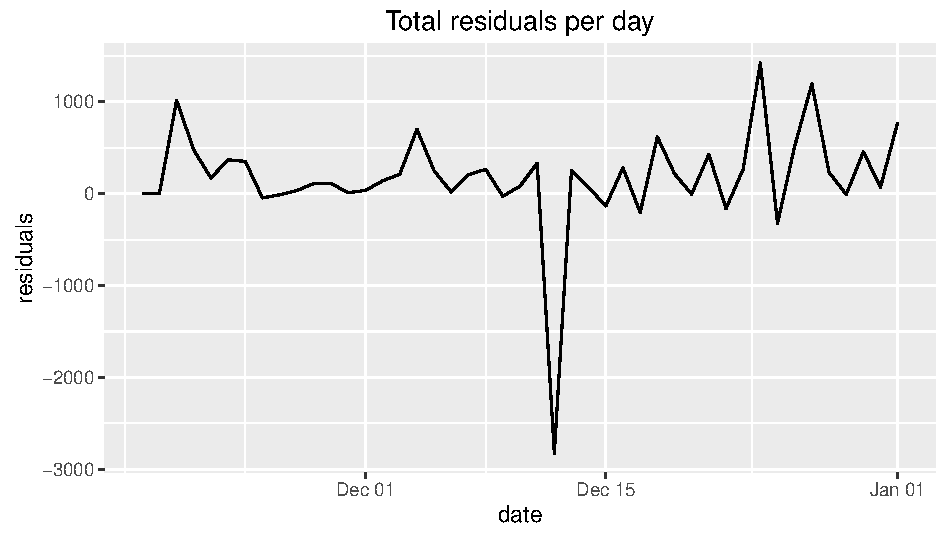
\includegraphics[width=0.49\textwidth]{Figures/Results/ResidualsTime}\label{fig:ResidualsTime}
}

\caption[Cluster model analysis]{Cluster model analysis. Figures  \ref{fig:resids} and \ref{fig:AbsPercErrLine} compare error and percentage error, the synthesised day 12-12-2011 is clearly visible as the blue outlier, Christmas eve and day, are shown in green and red respectively, and are not outliers despite what intuition might suggest. The scatter plot shown in figure \ref{fig:ActualVsPredErr}, visualises the error relative to a perfect fit shown as a black line. Figure \ref{fig:ErrDistrib} shows the right skewed error distribution caused primarily by the synthesised day 12-12-2011. The higher than average prediction error at 1900 seen in \ref{fig:AbsPercErrLine}, is reflect in in figure \ref{fig:BoxTimeErr}. Finally figure \ref{fig:ResidualsTime}, shows the daily total residual level across time, with the synthesised day a clear outlier.}
\label{fig:modanalysis}
\end{figure*}

\FloatBarrier

\subsection{Node cluster forecasting}
\label{sec:NodeClustforce}
As different clusters appeared on different days, only day pairs that had the same cluster set were used for testing the node cluster foreacasting, of which there were \hl{XXX} day pairs \hl{See table XXX, in the appendix for the days}. The results of the node clustering model indicated that the transition method is not effective for predicting the movement of individual nodes. The model returned and accuracy of 0.2627, or just over 1 in 4, across the 8 different clusters. However the $\kappa$ value was 0.1121 indicating that it was effectively random, in addition the p-value was 1, strongly suggesting the predictive power is nothing as a classifier. There is several reasons that the model results can be so poor, 1 is that the classifier will mark as fail, classifying into any adjacent cluster. Even though the clusters are temporally close because they are modelled as categorical values the closeness is irrelevant. A second complicating factor is that the two most probable clusters are 1630 and 2000, which are at opposite ends of the evening this means that small differences in percentage probability can mean large swings in cluster placement. 

As a comparison the model was compared to the XGboost algorithm this model had an accuracy of 0.3644 and a $\kappa$ of 0.1739 which is still low but considerably better than the transition model. The Xgboost model with the previous 7 days clusters had a slight improvement on the simple Xgboost model with an accuracy of 0.3689 and a $\kappa$ of 0.178, both of the XGboost models had a significant p-value, which the transition matrix method does not. The recent history provided by to the XGboost model gives it a large advantage, as if there is a pattern in moving between the nodes, the XGboost model would be able to pick it up where as the transition matrix would not. Overall the poor performance of both models suggests that the behaviour of the nodes as classified by the smart meters is very noisy, this is probably a combination of the low levels of consistent behaviour that were described in \ref{sec:basicconsum} and the hard classification of the clustering algorithm. However it does suggest that there will not be problems using a transition matrix generated from a different season than the predictions as there is no clear movement between clusters that could be affected by seasonal differences. 

A comparison of the Transition model and the XGboost model with 7 days cluster movement can be seen in \ref{fig:NodeClustFore}. The figure shows the relative accuracy of the two models. A perfect predictor woud have only the diagonal in red and everything else blue. The vertical bars exhibited by both models shows that they tend to miss-classify into the 1630 and 2000 classes, however the XGboost model has a much stronger diagonal which is reflects it's higher accuracy and $\kappa$ score.


\begin{figure*}[ht]
\centering
\subfloat[]{
  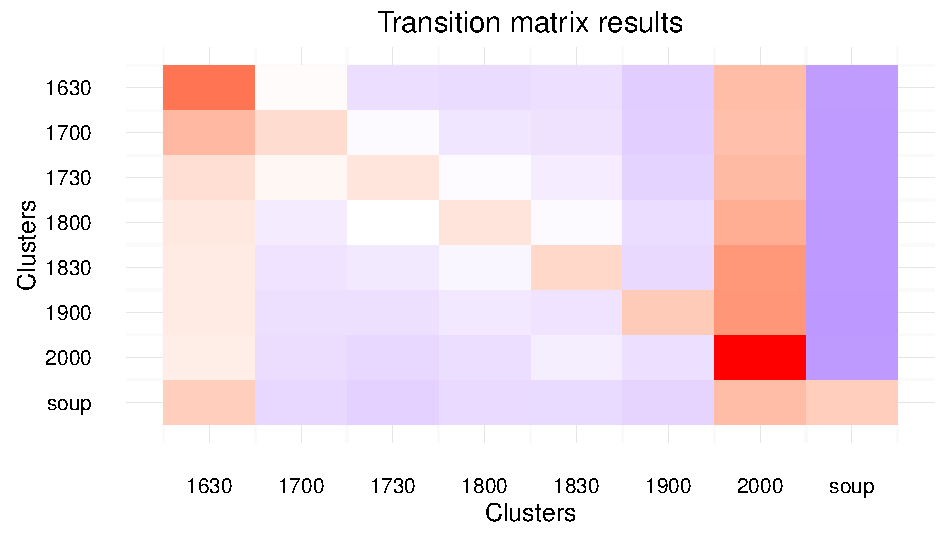
\includegraphics[width=0.49\textwidth]{Figures/Results/Transitionresults}\label{fig:NodeClustTrans}
}
\subfloat[]{
  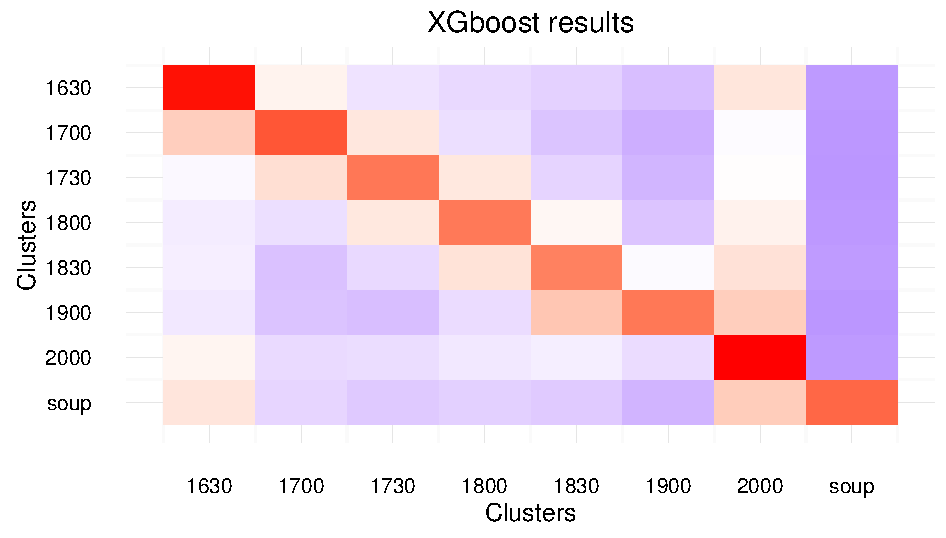
\includegraphics[width=0.49\textwidth]{Figures/Results/XGboostresults}\label{fig:NodeCLustXG}
}

\caption[Node Cluster Forecasting]{Visualising the accuracy of the Cluster transition matrix method and the XGboost method, it is clear that the XG boost method is more accurate with a much stronger diagonal than the cluster transition figure. Both clusters have higher errors on the 1630 and 2000 clusters this is likely simply because neither model is very accurate and so miss-classification ends up in these two clusters simply due to their relative size.}
\label{fig:NodeClustFore}
\end{figure*}

\subsection{Socio demographic detection}

The results of using XGboost to predict socio-demographic group based on probability of being in any given cluster did not perform any better than chance.  The accuracy of the overall model is 0.1665 and it had a $\kappa$ score close to zero,  the balanced accuracies of the individual classes was essentially 0.5 for every class. A major problem with the socio demographic detection is that the labels come from the mosaic cross classification system, where the classes of each area are based on demographic data for that area, as a result it can be noisy, making class detection difficult. In addition although there is some evidence that different social groups use energy in different ways, trying to detect it from such a small amount of data at the same time as using the experimental clustering technique may introduce too much noise to detect any signal that is actually there.

\section{Summary}

In this chapter the results of implementing chapter \ref{Method} are shown. Various decisions are made about the parameters of the analysis based on exploring the data, this includes having a minimum correlation requirement of 70\% for an edge in the graph and choosing the Louvain algorithm for clustering. In the 246 day time period, 8 clusters are detected including the Soup node, the clusters are primarily defined by the time of the mean peak of the cluster, the clusters discovered are 1630, 1700, 1730, 1800, 1830, 1900, 2000, and the node Soup. The predictive transition algorithm has a MAPE of 3.9\% which puts it on a par with other models seen in the literature and beats the linear predictor which had a MAPE of 5\%. Figures \ref{fig:ActualVsPredLine} and \ref{fig:ResidualsTime} showed that errors were induced when missing data was imputed, either in the form of raw data or clusters

The classification models that predicting the cluster of a node 1 day ahead were not as successful.The transition model had an accuracy of 25\% but a kappa score of 0.111 suggesting that it was not an effective model in comparison the XGboost models had all around better performance, the expanded XGboost model had an accuracy of 0.3689 and had a higher (but still low) $\kappa$ of 0.178, the results of these models suggest that there is a lot of noise in predicting day ahead nodes for individual smart meters. However the noisiness also suggests that using a transition matrix built with data from another season will not be a problem as if there is no pattern of movement between clusters at all there inherently cannot be any difference between seasons, therefore the transition matrix build time will not affect the results. The Socio-demographic detection was no better than random, this is likely to be due to noise in the MOSAIC classification and that socio-demographic class may not be a strong indicator of electricity consumption behaviour.






